\documentclass{beamer}

% for themes, etc.
\mode<presentation>
{ \usetheme{boxes} }

\usepackage{times}  % fonts are up to you
\usepackage{graphicx}

% Tikz
\usepackage{tikz}
\usetikzlibrary{calc}
\usetikzlibrary{arrows.meta}
\usetikzlibrary{intersections}
\usetikzlibrary{positioning}
\usetikzlibrary{shapes}
\usetikzlibrary{arrows}
\usetikzlibrary{fit}

\usepackage{xcolor, colortbl}
\usepackage{multirow}

\definecolor{LightGreen}{rgb}{0.5,0.8,0.5}
\definecolor{IntenseGreen}{rgb}{0.5,1,0.5}

\definecolor{LightYellow}{rgb}{0.82,0.81,0.58}
\definecolor{IntenseYellow}{RGB}{249,240,91}

\newcommand{\tuple}[1]{\ensuremath{\langle #1 \rangle}}
\newcommand{\type}[1]{\mathtt{#1}}
\newcommand{\personality}[5]{\tuple{\type{#1},\type{#2}, \type{#3}, \type{#4}, \type{#5}}}

% these will be used later in the title page
\title{Design and Implementation of an Agent Architecture combining Emotions and Reasoning}
\author{Janos Tapolczai\\ Matrikelnummer 0825077}
\date{Wien, 09.05.2016}

\setbeamertemplate{navigation symbols}{}%remove navigation symbols
\setbeamertemplate{footline}[frame number]

%\newlist{arrowlist}{itemize}{1}
%\setlist[arrowlist]{label=$\Rightarrow$}

% note: do NOT include a \maketitle line; also note that this title
% material goes BEFORE the \begin{document}

% have this if you'd like a recurring outline
\AtBeginSection[]  % "Beamer, do the following at the start of every section"
{
   \begin{frame}<beamer> 
      \frametitle{Content} % make a frame titled "Outline"
      \tableofcontents[currentsection]  % show TOC and highlight current section
   \end{frame}
}

\tikzset{
   every overlay node/.style={
      anchor=north west,
   },
}
% Usage:
% \tikzoverlay at (-1cm,-5cm) {content};
% or
% \tikzoverlay[text width=5cm] at (-1cm,-5cm) {content};
\def\tikzoverlay{%
   \tikz[baseline,overlay]\node[every overlay node]
}%

\begin{document}
   
   % this prints title, author etc. info from above
   \begin{frame}
      \titlepage
   \end{frame}
   
   \section{Our Goal}
   
   \begin{frame}{Our Goal}
         \begin{itemize}
            \item What is AI supposed to be able to do?
            \pause
            \item Many approaches based on search/logic exist:
               \begin{itemize}
                  \item A* search,
                  \item Iterated deepening DFS,
                  \item Answer-set programming, etc.
               \end{itemize}
            \pause
            \item These do well, but world-ontology has to be encoded in explicit rules!
         \end{itemize}
   \end{frame}

   \begin{frame}{Our Goal}
      \begin{itemize}
         \item Neural networks are another approach:
         \begin{itemize}
            \item supervised learning,
            \item unsupervised learning,
            \item hierarchical learning, etc.
         \end{itemize}
         \pause
         \item The network must approximate some function with the help of training data.
         \pause
         \item We must have labelled examples/cost functions available.
         \pause
         \item It's not obvious what a neural network ``understands''.
      \end{itemize}
   \end{frame}
   
   \begin{frame}{Our Goal}
      
      \begin{itemize}
         \item We want to closely imitate the biological brain.
         
         \pause
         
         \item We are interested in
         \begin{itemize}
            \item \emph{realistic behaviour}
            \item and \emph{realistic cognition}.
         \end{itemize}
         
         \pause
         
         \item Our inspirations:
         \begin{itemize}
            \item \emph{evolutionary neurobiology} and
            \item nouvelle AI.
         \end{itemize}
      \end{itemize}
   \end{frame}
   
   \begin{frame}{Our Goal --- Nouvelle AI}
      
         \pause
      
         \begin{quote}\emph{
            One aim of nouvelle AI is the relatively modest one of producing systems that display the same level of intelligence as insects.
         }\end{quote}
         
         \pause
            
        \begin{quote}\emph{
           A central idea of nouvelle AI is that the basic building blocks of intelligence are very simple behaviours {\upshape[$\dots$]} More complex behaviours ``emerge'' from the interaction of these simple behaviours.
         }\end{quote}
         
         \pause
         
         Jack Copeland. What is Artificial Intelligence?\\
         {\footnotesize\url{http://www.alanturing.net/turing_archive/pages/Reference\%20Articles/what\_is\_AI/What\%20is\%20AI11.html}}
   \end{frame}
   
   \begin{frame}{Our Goal --- Evolutionary Neurobiology}
      
      \begin{itemize}
         \item In what order did the components of the brain evolve?
         \item What is their relation to each other?
         \item How well is the brain ``designed''?
      \end{itemize}
      
      \pause
      
      \begin{quote}\emph{
            It is not worth asking how to define consciousness, how to explain it, how it
            evolved, what its function is, etc., because there’s no one thing for which all
            the answers would be the same. Instead, we have many sub-capabilities, for
            which the answers are different: e.g., different kinds of perception, learning,
            knowledge, attention control, self-monitoring, self-control, etc.
         }\end{quote}

         Aaron Sloman, quoted in \emph{The Emotion Machine}, p. 97.
         \end{frame}
   
   \section{Biological Considerations}
   
   \begin{frame}{Biological Considerations}
      \begin{itemize}
            \item Nervous systems long predate brains.
            \item Brains themselves evolved over hundreds of millions of years.
      \end{itemize}
   \end{frame}
   
   \begin{frame}{Biological Considerations}
      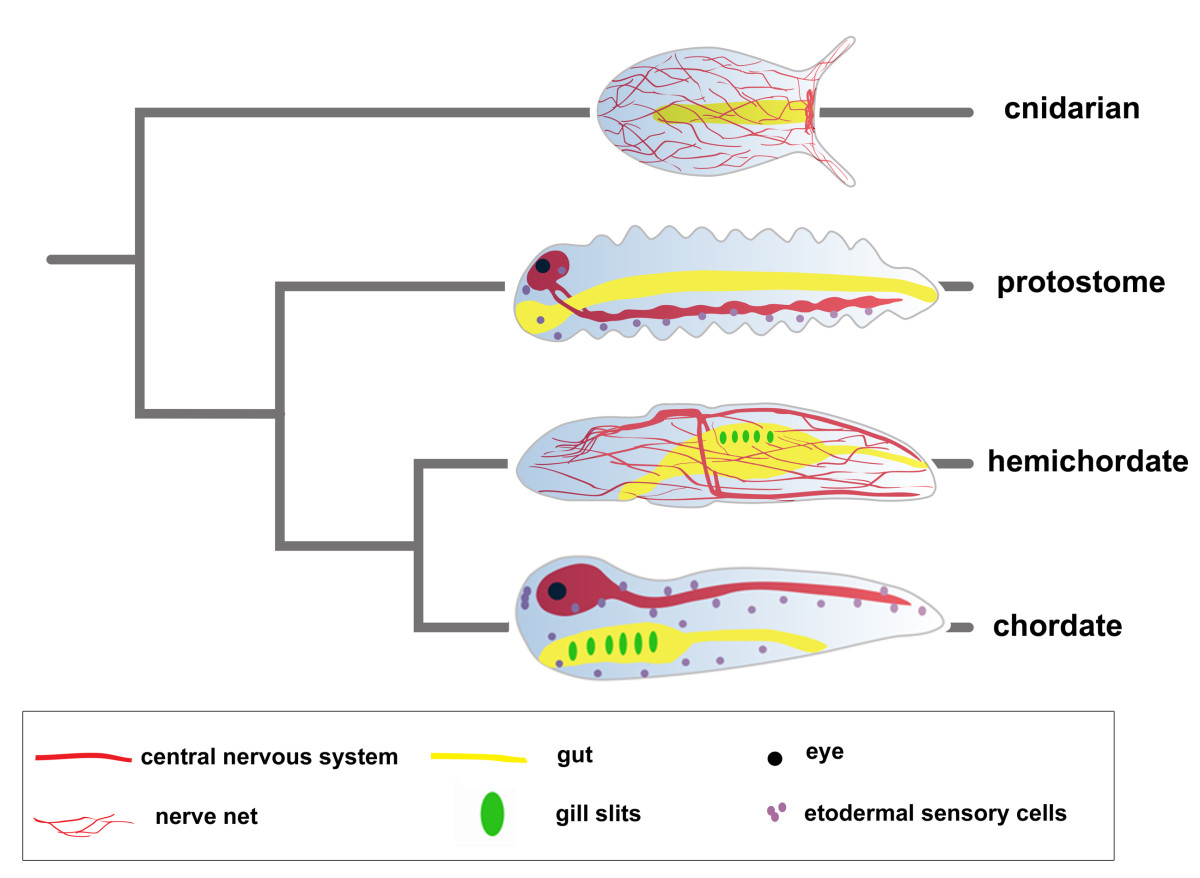
\includegraphics[width=\textwidth]{../Thesis/Figs/chordata.jpg}
   \end{frame}

   \begin{frame}{Biological Considerations}
      \begin{itemize}
         \item Neurons function as a signalling mechanism in an organism.
         \pause
         \item They receive signals from body parts, but also other neurons.\\
            $\Rightarrow$ Neurons \emph{listen in} on other neurons.
         \pause
         \item Functionality was added gradually, with no long-term design.\\
            $\Rightarrow$ Components have no well-defined interfaces.
         \pause
         \item Thus our working hypothesis: a \emph{White-box model of cognition}.
       \end{itemize}
   \end{frame}
   
   \begin{frame}{Biological Considerations - White-box model}
      \begin{itemize}
         \item Traditional programming languages work via \emph{black boxes}:\\
              \vspace{2mm}
               A functions are called, but their internals are unobservable.
               \vspace{2mm}
         \item We assume that components in the brain are \emph{white boxes}:\\
              \vspace{2mm}
               Any component can observe the activity of others.
      \end{itemize}
   \end{frame}
   
   \begin{frame}{Biological Considerations - White-box model}
      \begin{itemize}
         \item Of course, practical considerations apply.
         \vspace{2mm}
         \item We still use regular functions within components,
         \item but components can publish \emph{messages}.
         \item These are stored in a central \emph{message space}.
         \item Any component can read from and write into the message space.
         \vspace{2mm}
         \item Components are \emph{loosely coupled}:\\
            $\Rightarrow$ components don't know who reads their messages;\\
            $\Rightarrow$ components don't know who wrote the messages.
      \end{itemize}
   \end{frame}
   
   \section{Architecture}
   
   \begin{frame}{Architecture}
       \begin{itemize}
          \item The implementation consists of a
             \begin{itemize}
                \item \emph{world simulator} and an
                \item \emph{agent architecture}.
             \end{itemize}
       \end{itemize}
   \end{frame}
   
   \begin{frame}{Architecture --- World Simulator}
      \begin{itemize}
         \item Worlds are 2D grids with some inaccessible cells.
         \item \emph{Entities} are agents or Wumpuses.
         \item \emph{Wumpuses} roam the world in search for agents.
       \item \emph{Meat}, \emph{fruits}, and \emph{gold} lie around.
         \item \emph{Plants} can be harvested for fruit.
         \item Killed entitites leave behind meat.
         
         \vspace{2mm}
         \item Pits kill whatever falls into them.
         \vspace{2mm}
         \item Entities can fight, but this costs health.
         \item Meat and fruit can be \emph{eaten} to restore health.
         \item Agents can give each other gifts and communicate via gestures.
      \end{itemize}
   \end{frame}
   
   \begin{frame}{Architecture --- World Simulator}
      \begin{itemize}
         \item Time moves in rounds.
         \item In each round, every entity takes one action.
            \begin{itemize}
               \item The entity gets a slice of the world as \emph{perception} and
               \item it has to return its desired action.
            \end{itemize}
         \item Actions are
            \begin{itemize}
               \item \emph{move},
               \item \emph{rotate},
               \item \emph{attack},
               \item \emph{gather},
               \item \emph{eat}, etc.
            \end{itemize}
      \end{itemize}
   \end{frame}
   
   \begin{frame}{Architecture --- Agents}
      \begin{itemize}
            \item Based on evolutionary considerations, we designed 7 components.
            \vspace{2mm}
            \item Perception,
            \item Pre-social Behaviour Control (PSBC),
            \item Social Judgment System (SJS),
            \item Memory,
            \item Attention Control (AC),
            \item Decision Maker (DM), and
            \item Belief Generator (BG).
      \end{itemize}
      
      \tikzoverlay at (7.8cm,0.3cm) {
         \tikz node (label) at (0,0)[]{
            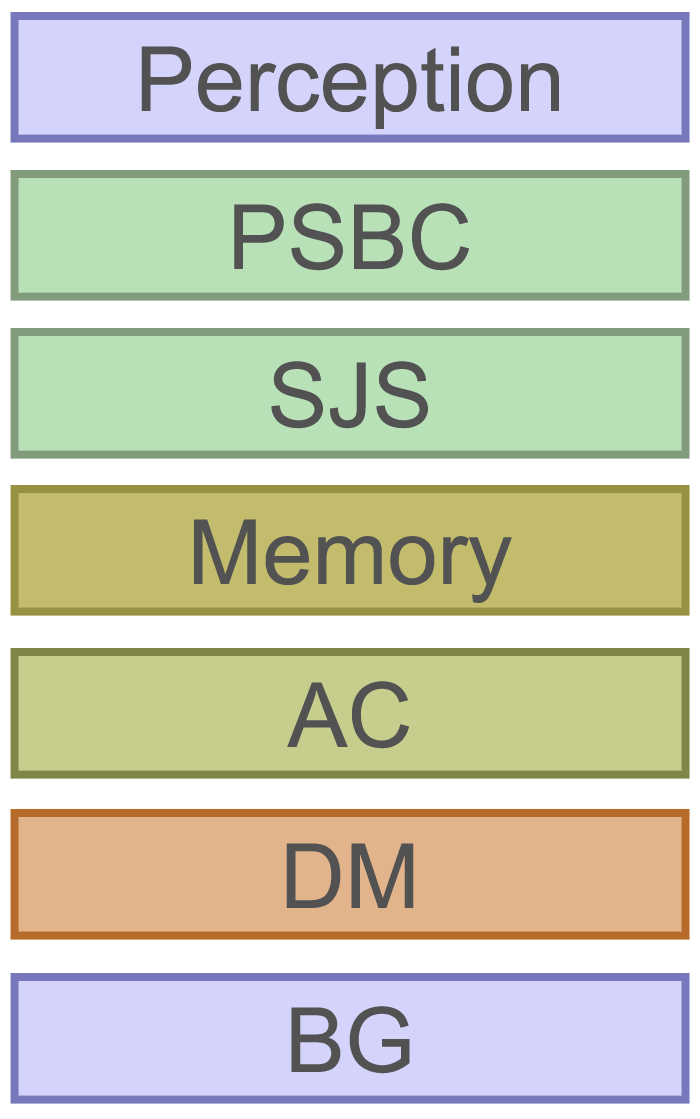
\includegraphics[width=3cm]{agent_components_intense.png}
         };
      };
   \end{frame}
   
   \begin{frame}{Architecture --- Agents}
      \begin{itemize}
         \item Perception
            \begin{itemize}
               \item Complex messages from the world simulator are chopped up into atomic pieces.
               \item The other components only have to deal with simple facts, e.g.
                  \begin{itemize}
                     \item ``My Health is 0.7'',
                     \item ``Cell (x,y) has an entity'', or
                     \item ``There is a plant on cell (x,y)''.
                  \end{itemize}
            \end{itemize}
      \end{itemize}
      
%      \tikzoverlay[text width=1.8cm] at (9.7cm,3.9cm) {
%         \tikz node (label) at (0,0)[]{
%            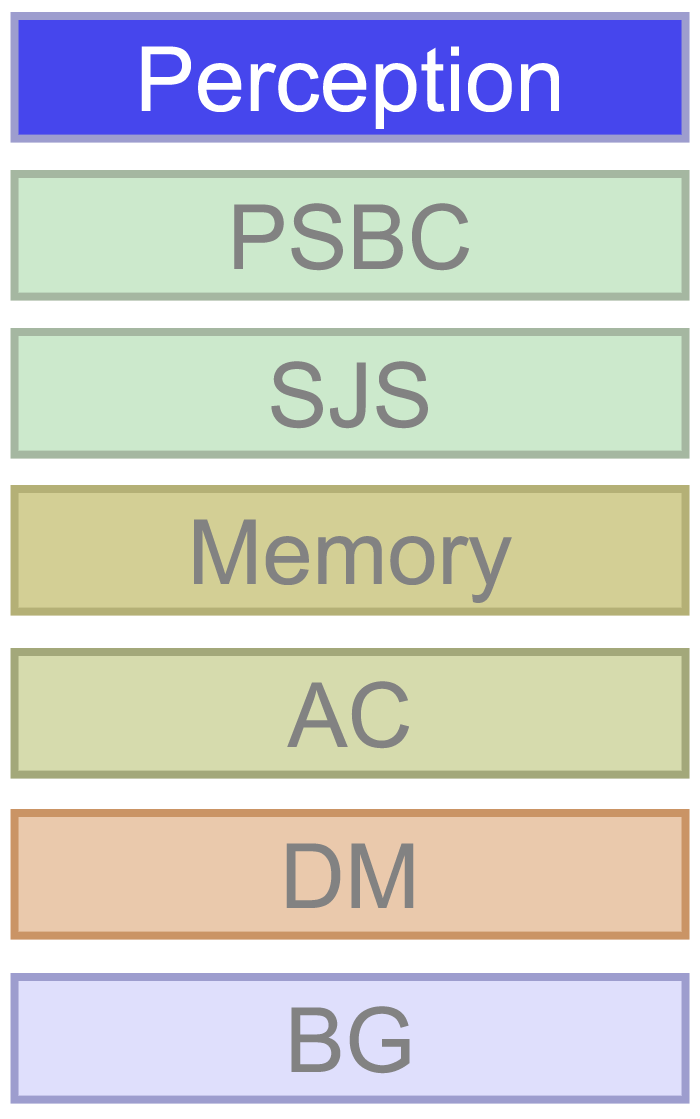
\includegraphics[width=1.8cm]{agent_components_perception.png}
%         };
%      };
   \end{frame}
   
   \begin{frame}{Architecture --- Agents}
      \begin{itemize}   
         \item Pre-Social Behaviour Control
         \pause
            \begin{itemize}
               \item The agent has four emotions:
                  \begin{itemize}
                     \item anger,
                     \item fear,
                     \item enthusiasm, and
                     \item contentment.   
                  \end{itemize}
               \pause
               \item Each emotion has an associated graph.
               \pause
               \item Each node responds to a specific message (e.g. low health).
               \pause
               \item Nodes may activate neighboring nodes.
               \pause
               \item The more nodes are activated, the stronger the emotion.
               \pause
               \vspace{3mm}
               \item ``Pre-Social'' $\Rightarrow$ anger, fear, etc. are evolutionarily older than social emotions like trust or contempt.
            \end{itemize}
      \end{itemize}
      
%      \tikzoverlay[text width=1.8cm] at (9.7cm,3.9cm) {
%         \tikz node (label) at (0,0)[]{
%            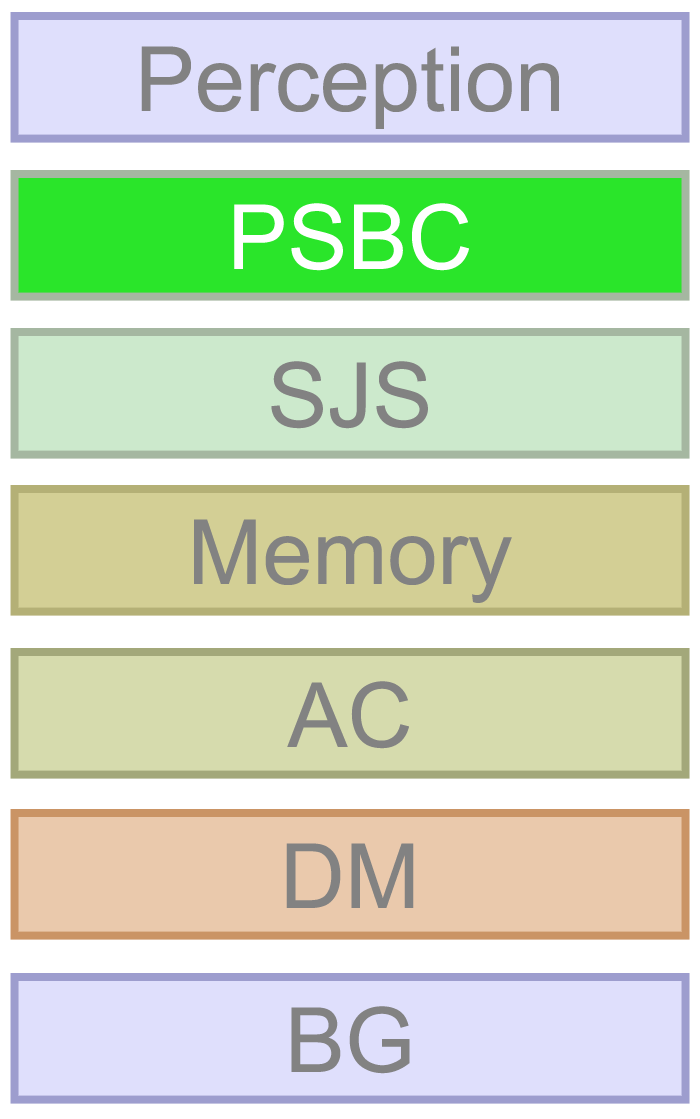
\includegraphics[width=1.8cm]{agent_components_psbc.png}
%         };
%      };
   \end{frame}
   
   \begin{frame}{Architecture --- Agents}
      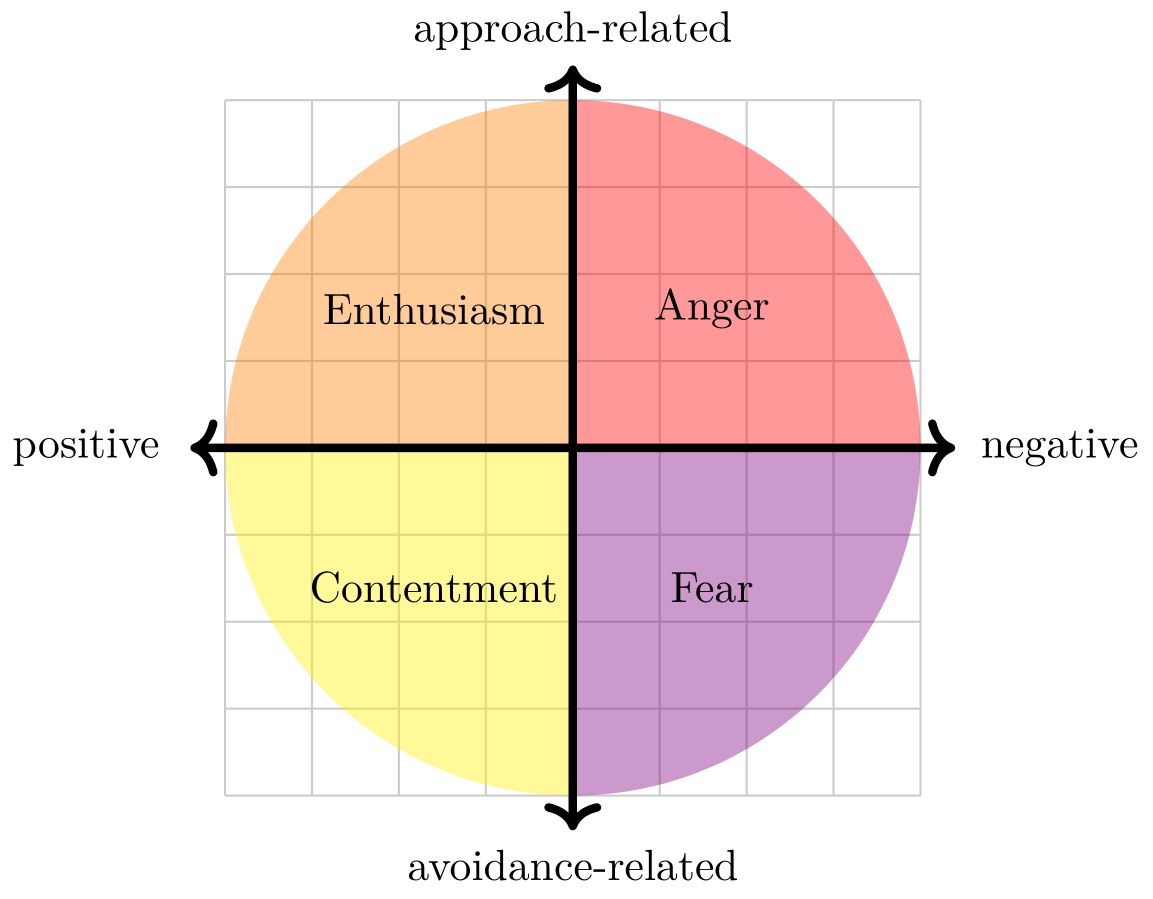
\includegraphics[width=\textwidth]{../Thesis/Figs/PSBC.png}
   \end{frame}
   
   \begin{frame}{Architecture --- Agents}
      \begin{itemize}
         \item {Social Judgment System}
            \begin{itemize}
               \item Other agents evoke
                  \begin{itemize}
                     \item sympathy,
                     \item trust,
                     \item respect.
                  \end{itemize}
               \pause
               \item Every stranger has its own emotional levels.
               \item Agents can become friends (through positive interactions) or enemies.
            \end{itemize}
      \end{itemize}
      
%      \tikzoverlay[text width=1.8cm] at (9.7cm,3.9cm) {
%         \tikz node (label) at (0,0)[]{
%            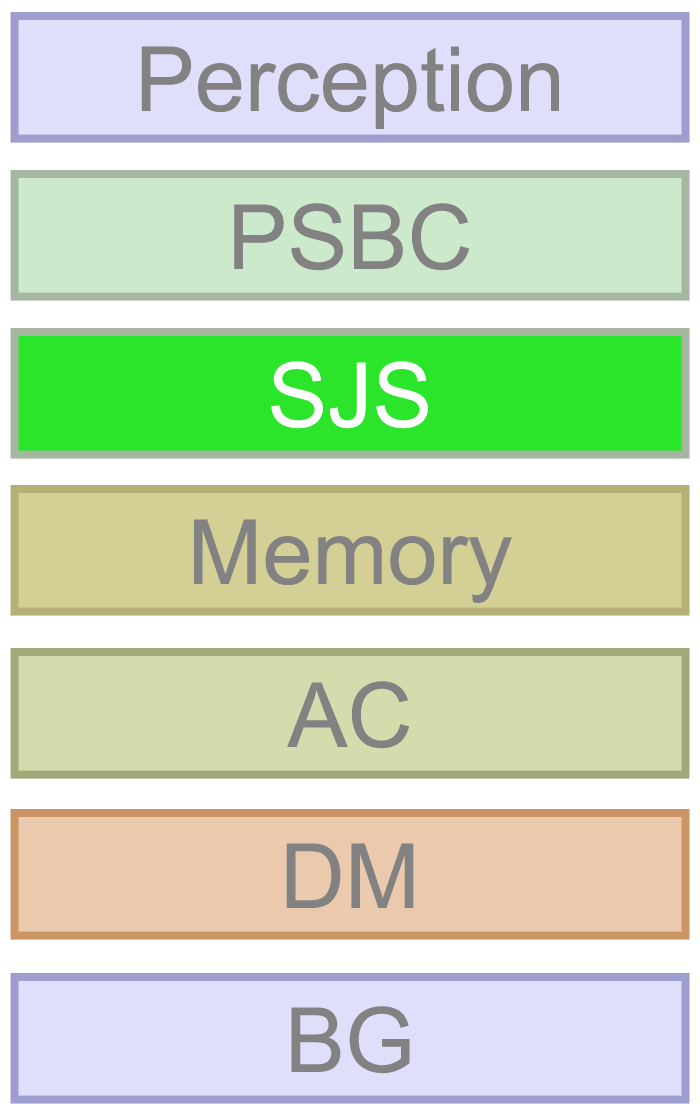
\includegraphics[width=1.8cm]{agent_components_sjs.png}
%         };
%      };
   \end{frame}
   
   \begin{frame}{Architecture --- Agents}
      \begin{itemize}
         \item Memory
         \begin{itemize}
            \item We store our perceptions for later recall.
            \item Memory can also store \emph{imagined} worlds in a \emph{tree structure}.
         \end{itemize}
         \pause
         \item Attention Control
         \begin{itemize}
            \item We assist the Decision Maker by selecting important targets.
            \item ``Important'' means ''evokes the strongest emotions''.
         \end{itemize}
      \end{itemize}
      
%      \tikzoverlay[text width=2cm] at (9.5cm,3.3cm) {
%         \tikz node (label) at (0,0)[]{
%            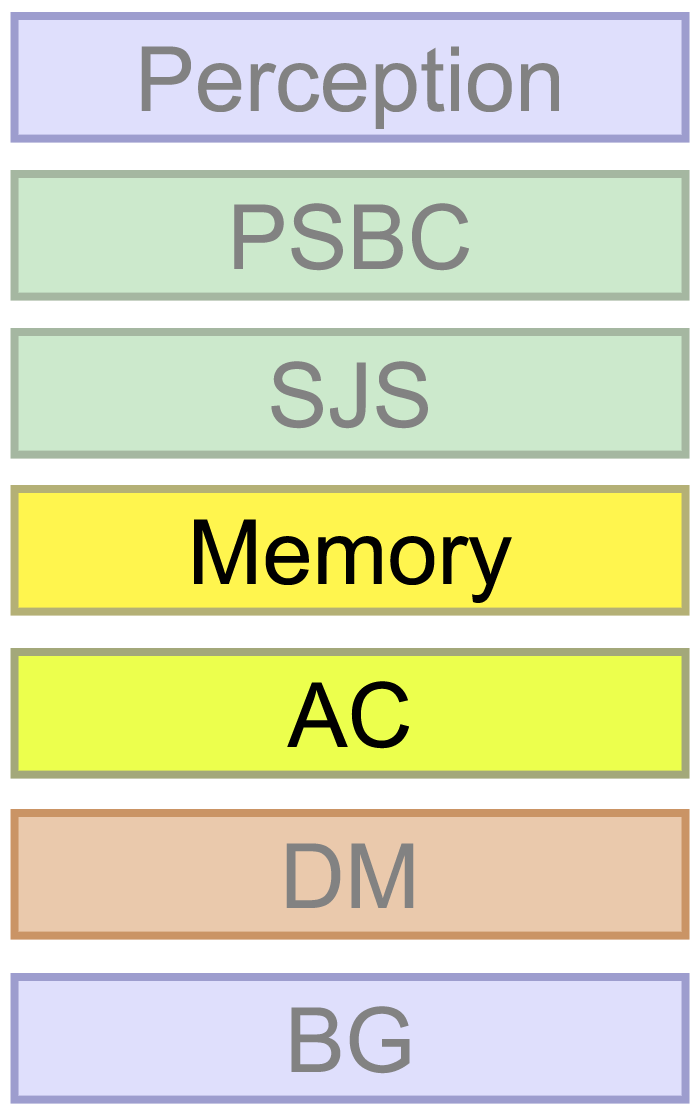
\includegraphics[width=2cm]{agent_components_memory_ac.png}
%         };
%      };
   \end{frame}
   
   \begin{frame}{Architecture --- Agents}
      \begin{itemize}
         \item Decision Maker
            \begin{itemize}
               \item Each emotion has some actions associated with it, e.g.,
               \begin{itemize}
                  \item attacking is associated with anger,
                  \item eating is associated with enthusiasm.
               \end{itemize}
               \pause
               \item The PSBC and the AC guide the planning:
               \begin{itemize}
                  \item We select an action associated with our strongest emotion,
                  \item and the cell(s) which have the most attention.
               \end{itemize}
               \pause
               \item If our emotion is strong enough, we take a \emph{real} action,
               \item otherwise, we take a \emph{hypothetical} one.
               \vspace{2mm}
               \item The DM can also abort plans if, e.g., fear begins to override anger.
            \end{itemize}
      \end{itemize}
      
%      \tikzoverlay[text width=1.8cm] at (9.7cm,3.9cm) {
%         \tikz node (label) at (0,0)[]{
%            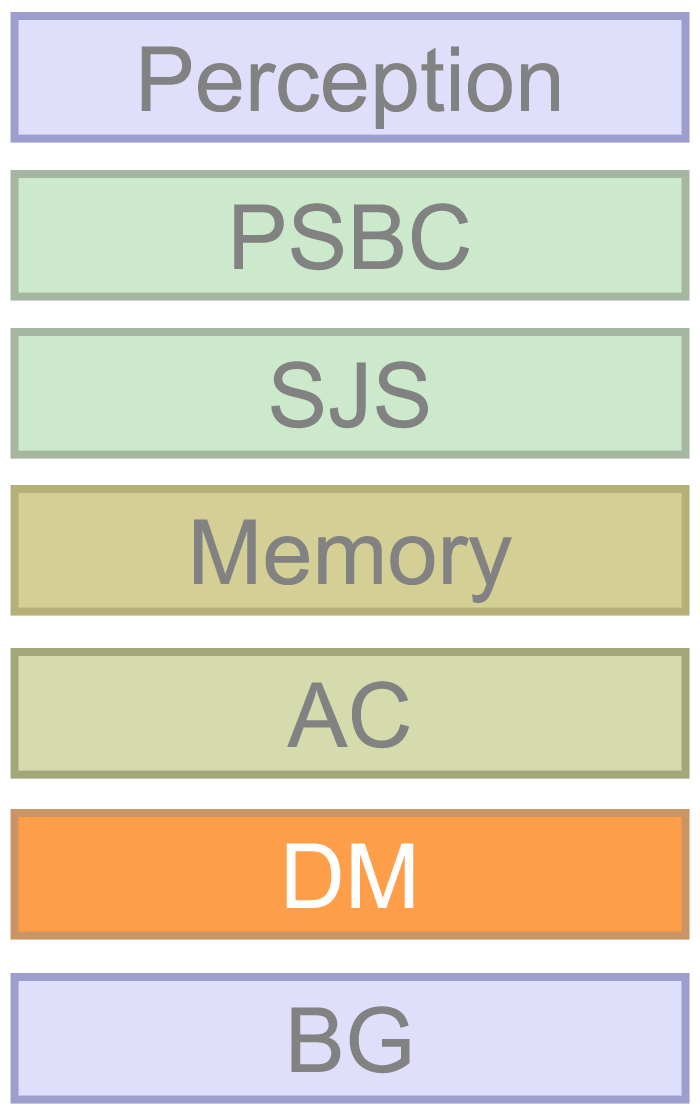
\includegraphics[width=1.8cm]{agent_components_dm.png}
%         };
%      };
   \end{frame}
   
   \begin{frame}{Architecture --- Agents}
      \begin{itemize}
         \item Belief Generator
         \begin{itemize}
            \item If the DM chose a \emph{hypothetical} action, we simulate its consequences.
            \item We use the actual world simulator, but we construct the world from memory.
            \item The agent is then given \emph{imagined perceptions}.
         \end{itemize}
      \end{itemize}
      
%      \tikzoverlay[text width=1.8cm] at (9.7cm,3.9cm) {
%         \tikz node (label) at (0,0)[]{
%            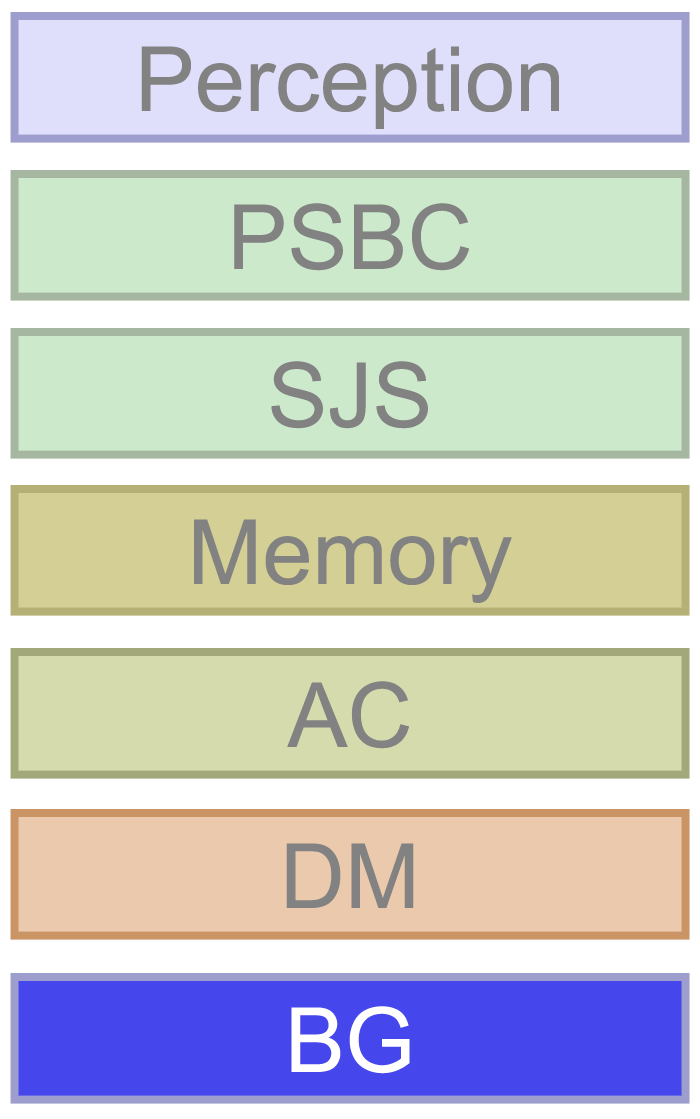
\includegraphics[width=1.8cm]{agent_components_bg.png}
%         };
%      };
   \end{frame}
   
   \begin{frame}{Architecture --- Agents}
      \begin{itemize}
         \item {How does this all fit together?}
      \end{itemize}
      
      \begin{center}
         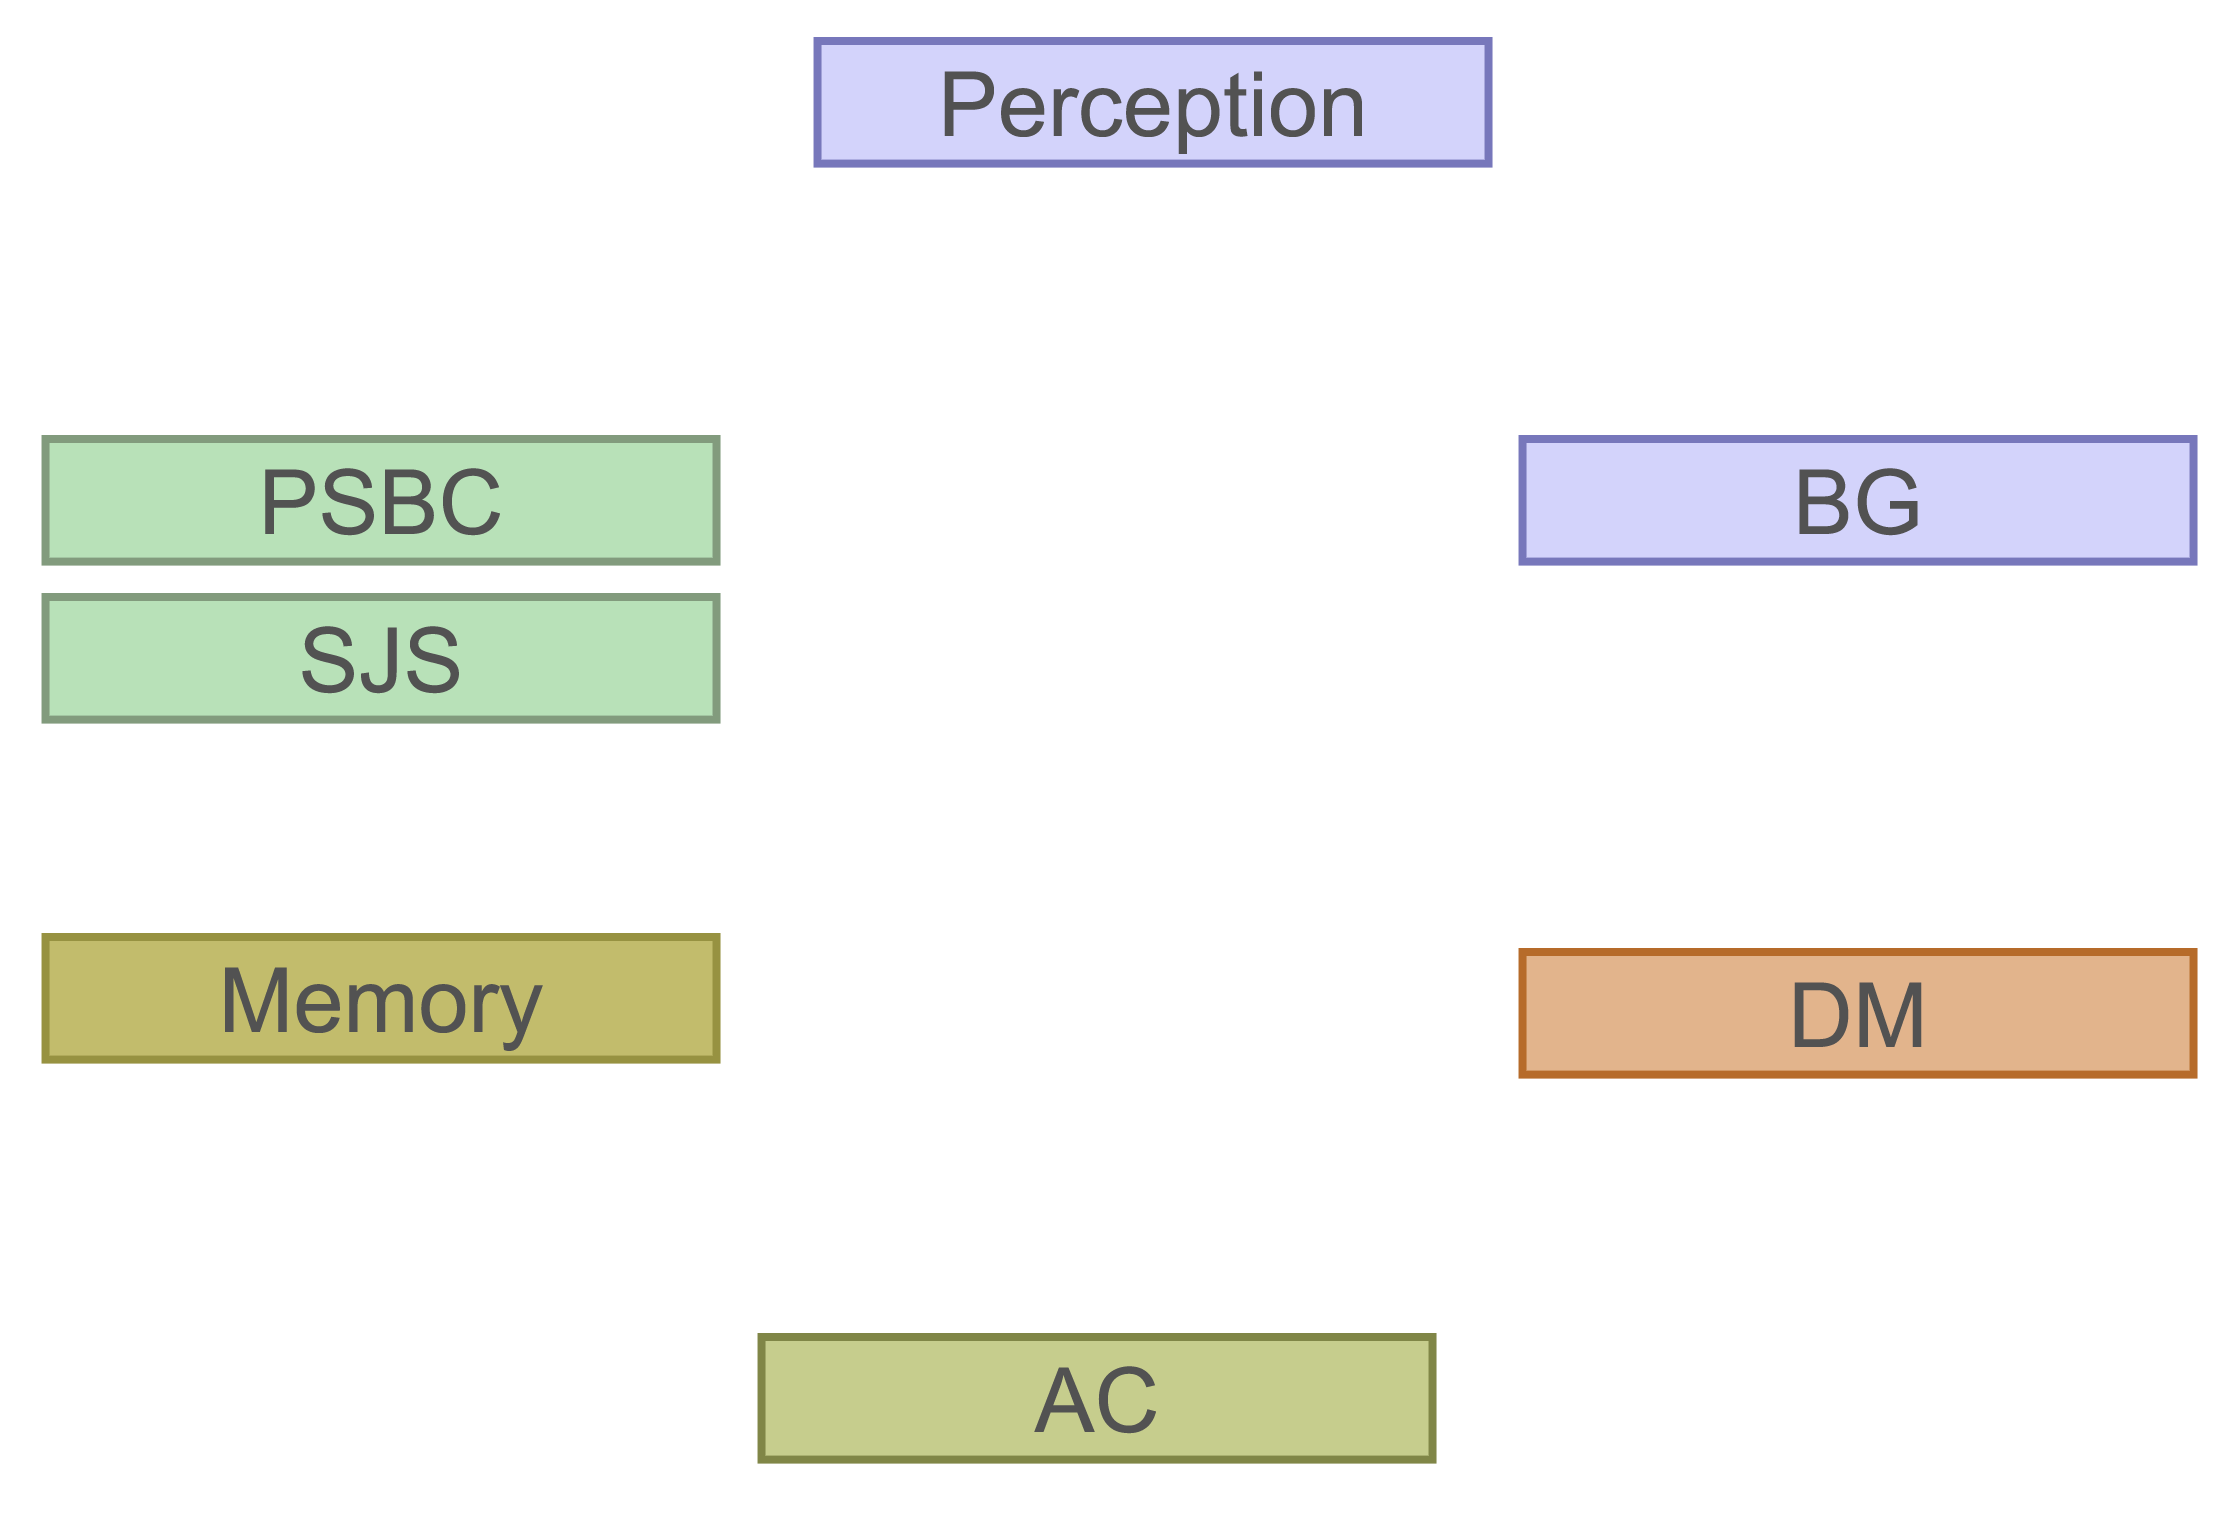
\includegraphics[width=0.8\textwidth]{plan_0.png}
      \end{center}
      
      ~
   \end{frame}
   
   \begin{frame}{Architecture --- Agents}
      \begin{itemize}
         \item {How does this all fit together?}
      \end{itemize}
      
      \begin{center}
         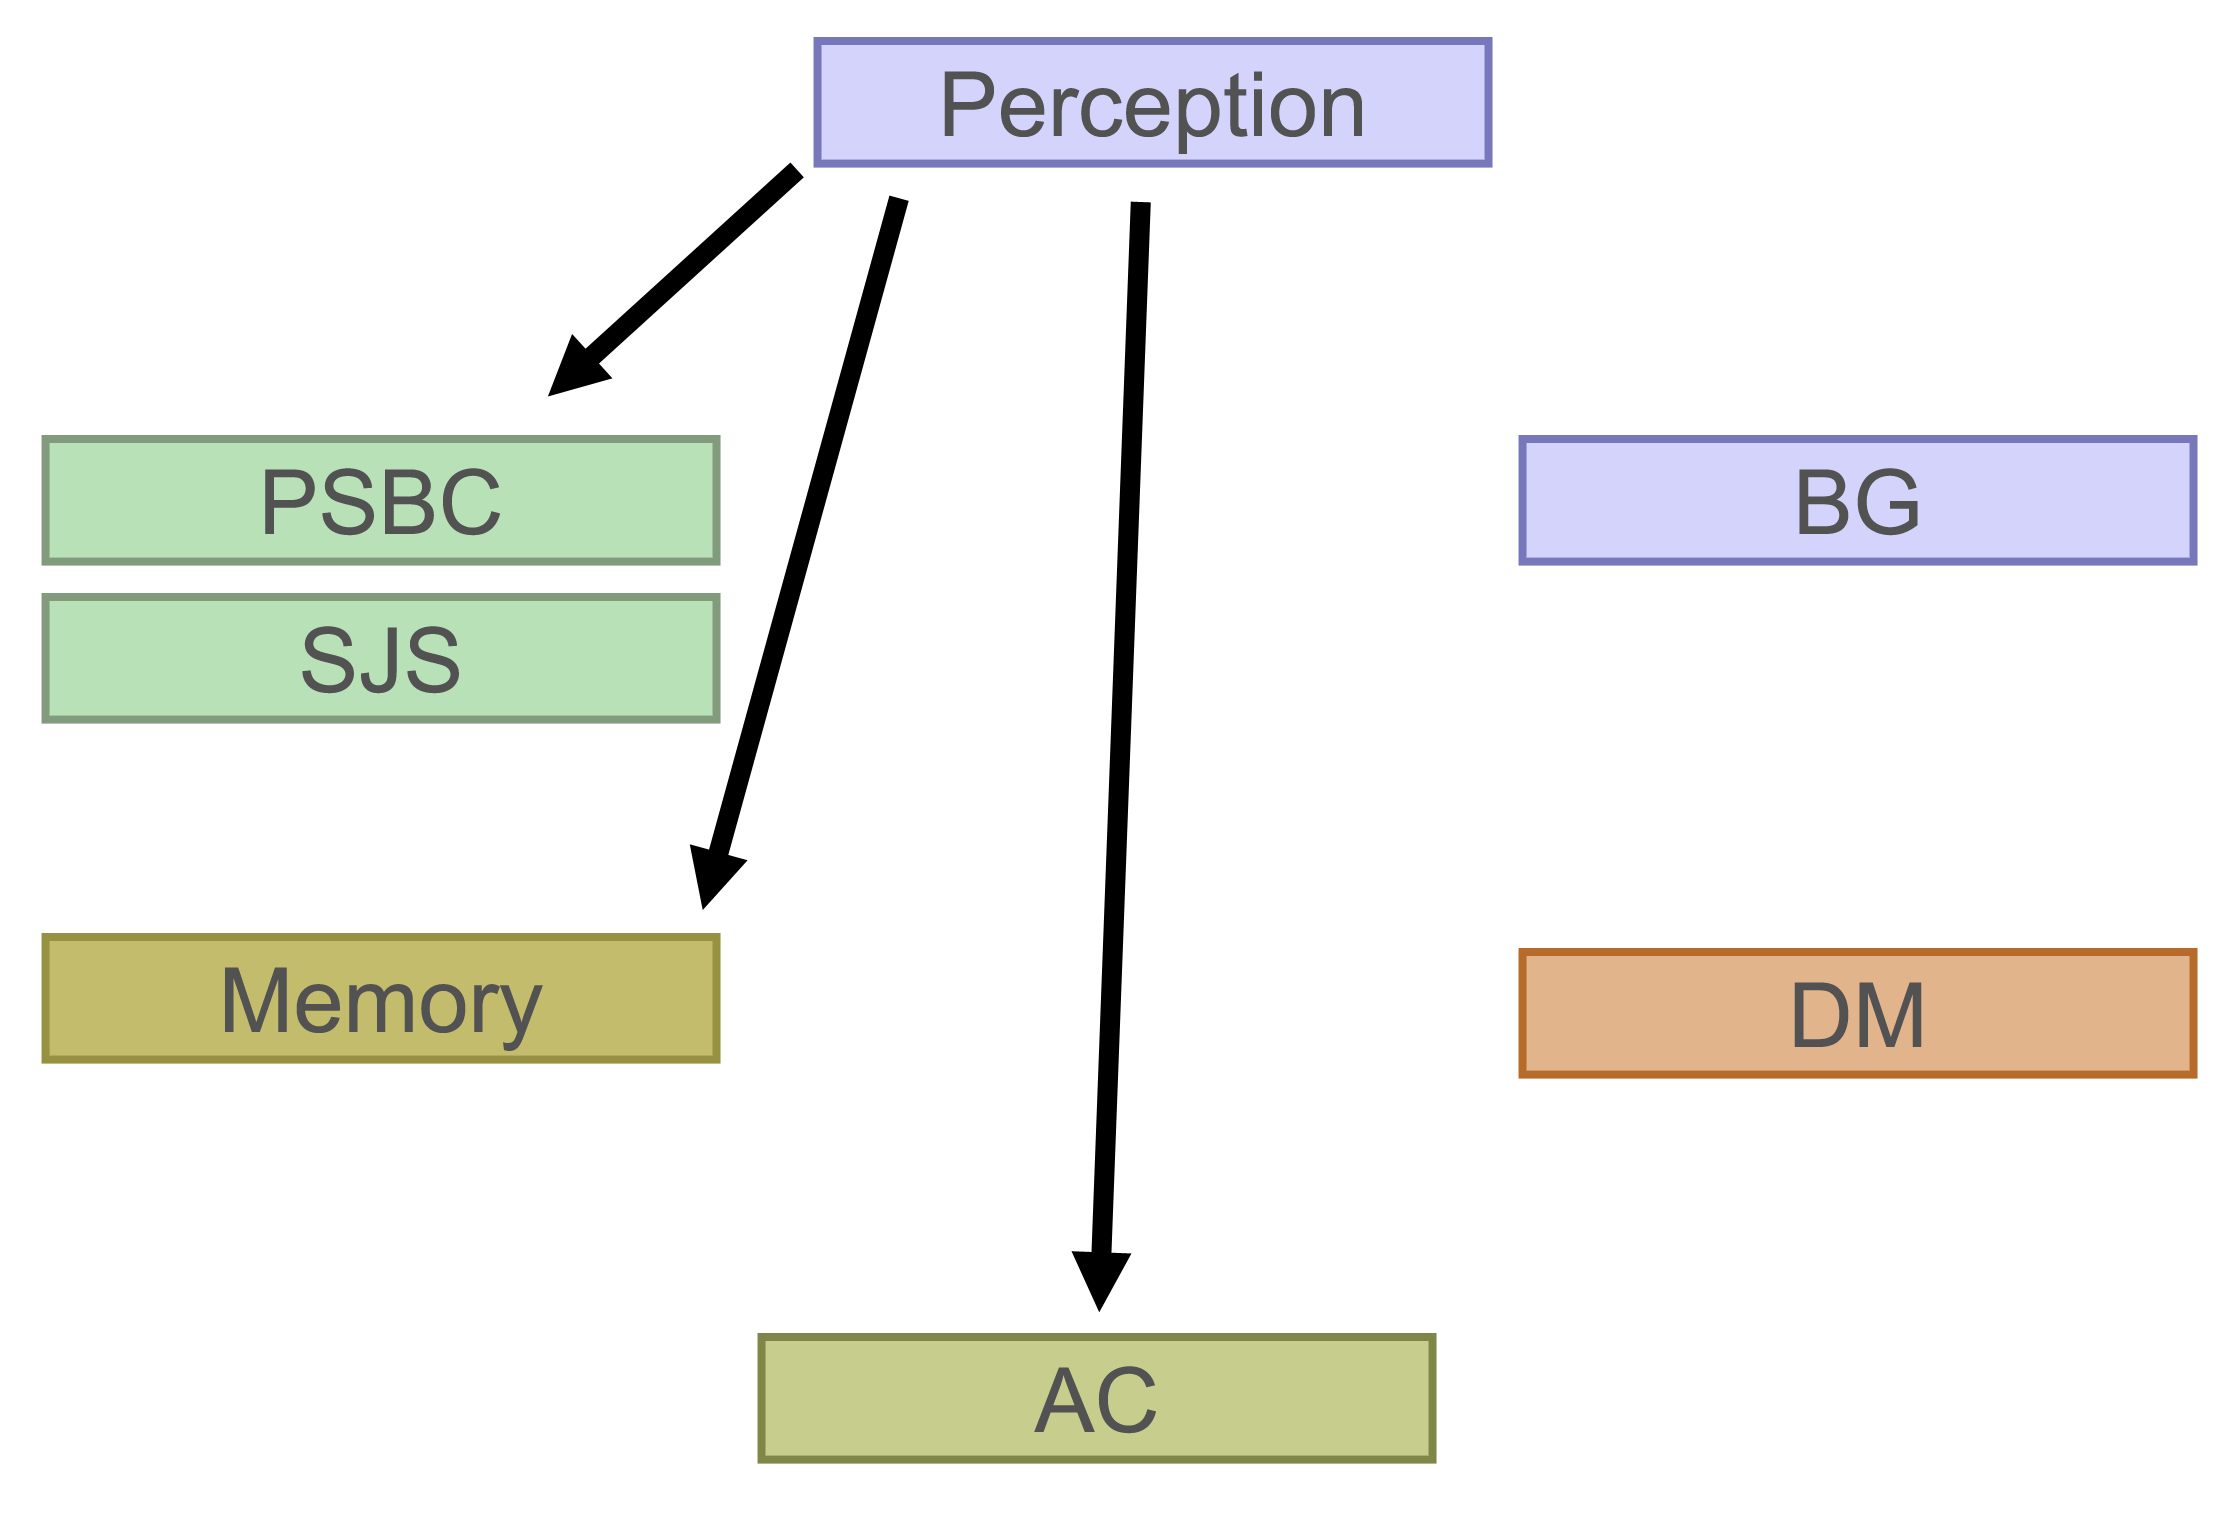
\includegraphics[width=0.8\textwidth]{plan_1.png}
      \end{center}
      
      \emph{Perception} distributes its messages.
   \end{frame}
   
   \begin{frame}{Architecture --- Agents}
      \begin{itemize}
         \item {How does this all fit together?}
      \end{itemize}
      
      \begin{center}
         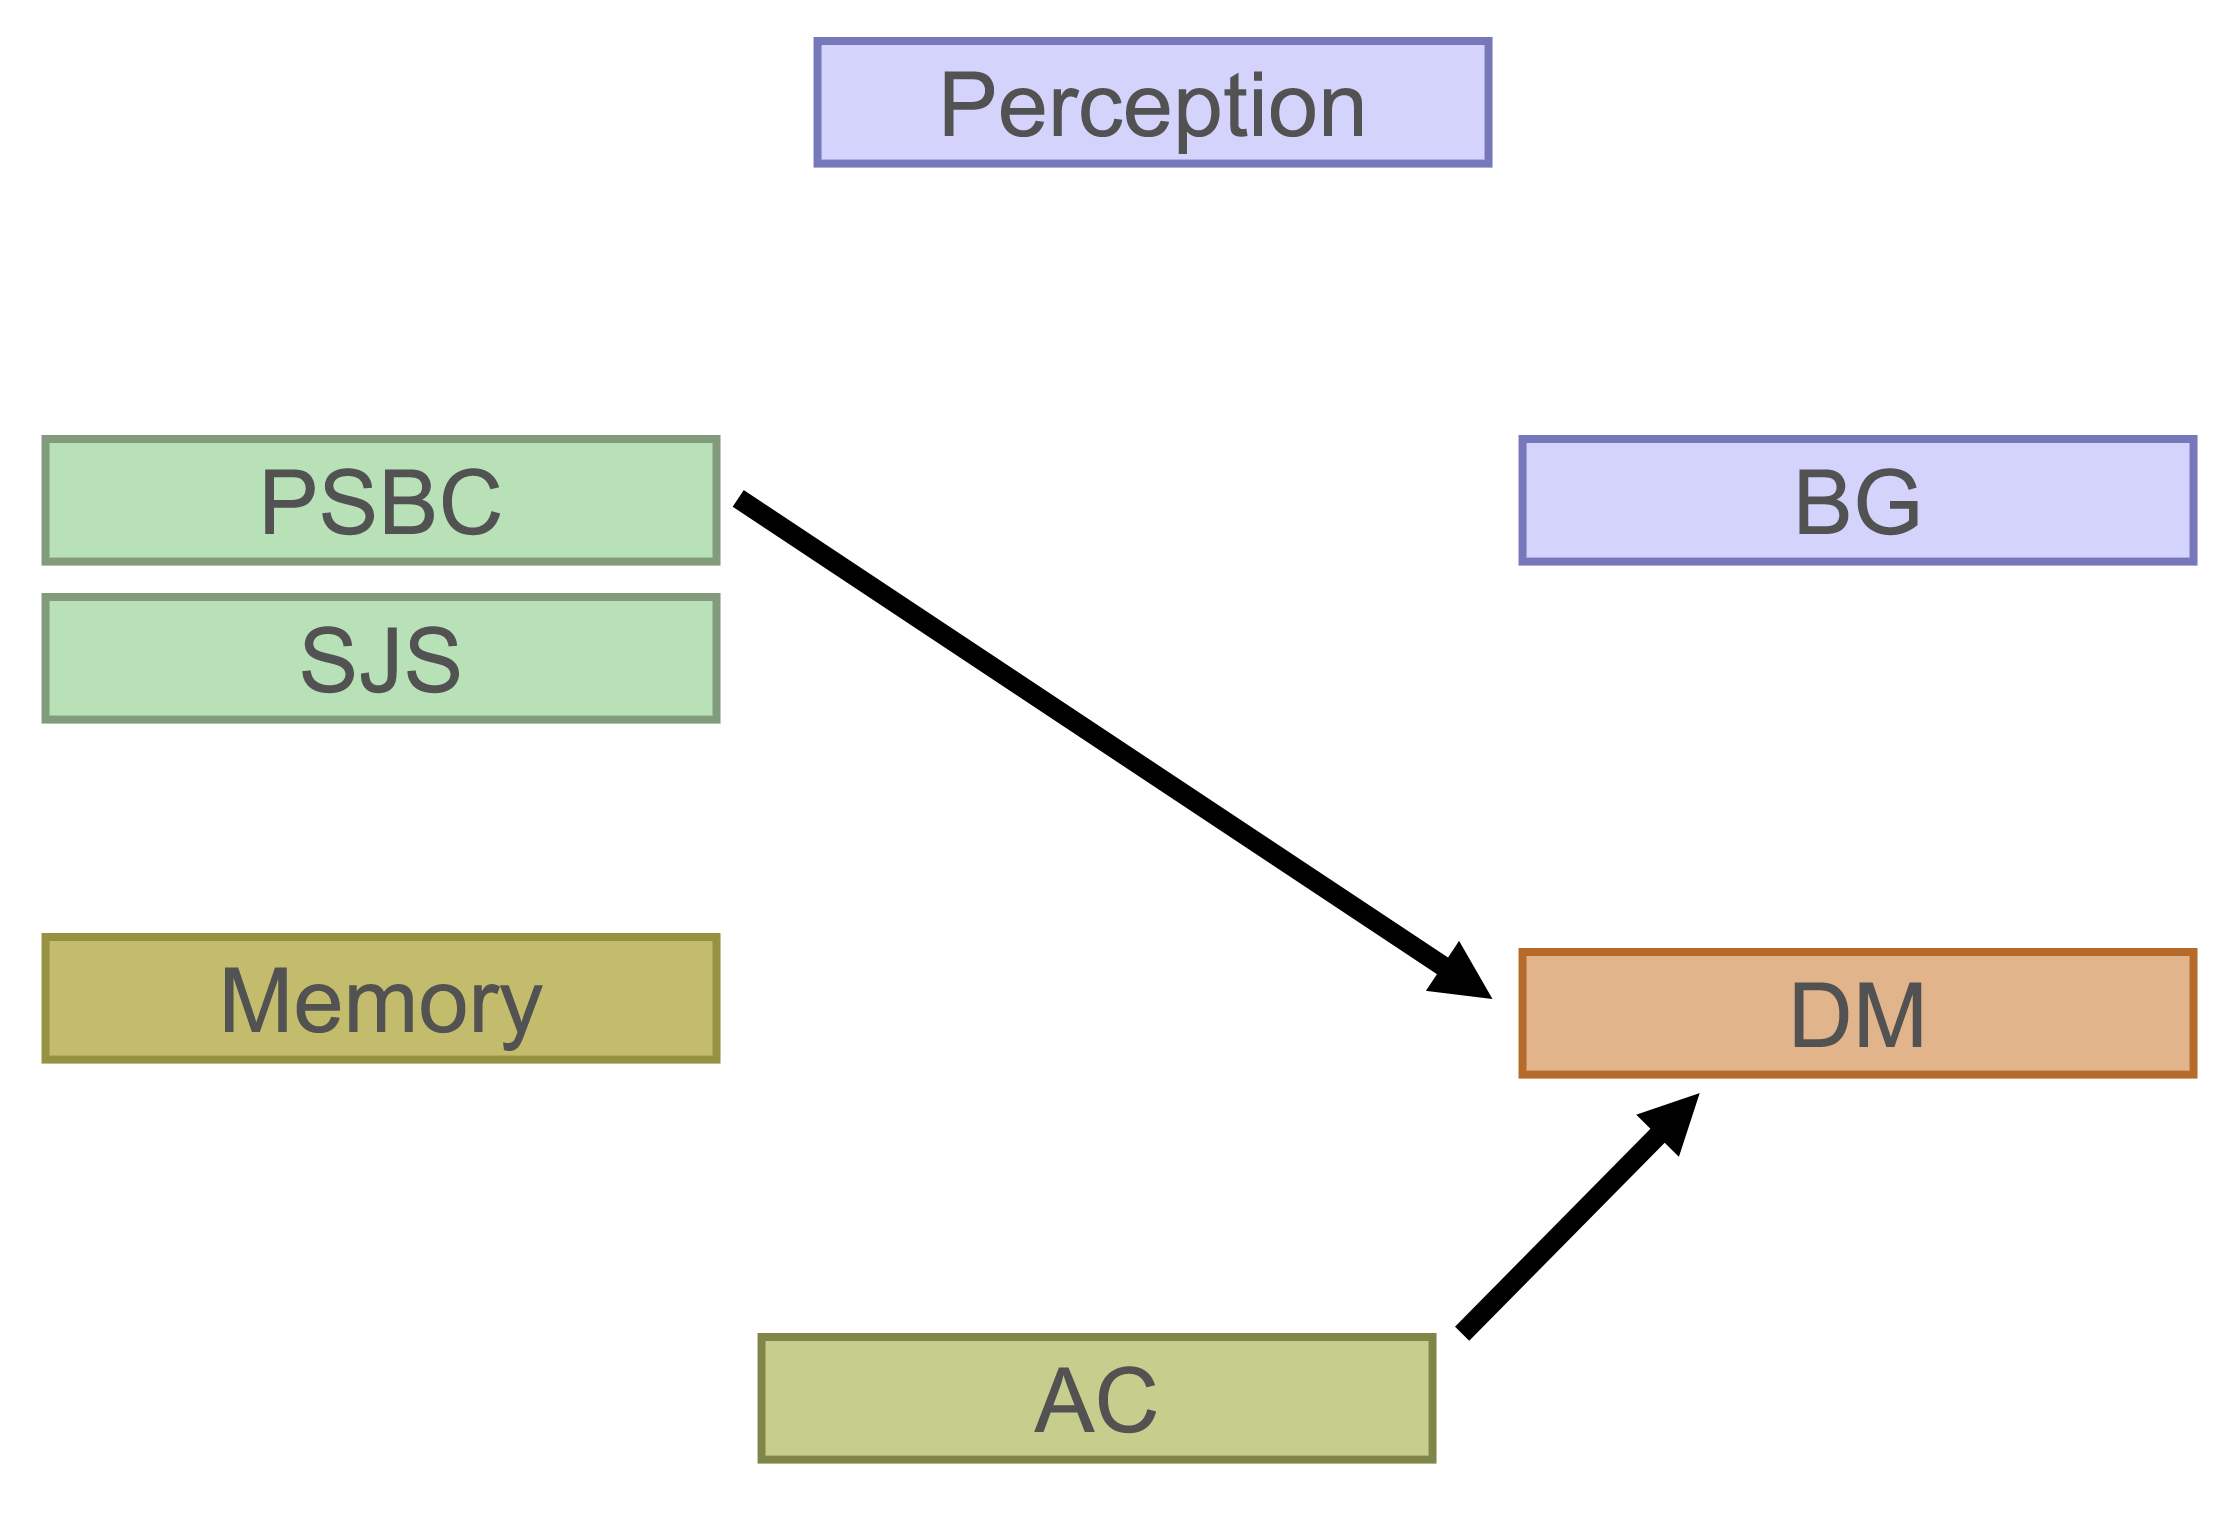
\includegraphics[width=0.8\textwidth]{plan_2.png}
      \end{center}
      
      The \emph{Decision Maker} is informed about the affective reactions.
   \end{frame}
   
   \begin{frame}{Architecture --- Agents}
      \begin{itemize}
         \item {How does this all fit together?}
      \end{itemize}
      
      \begin{center}
         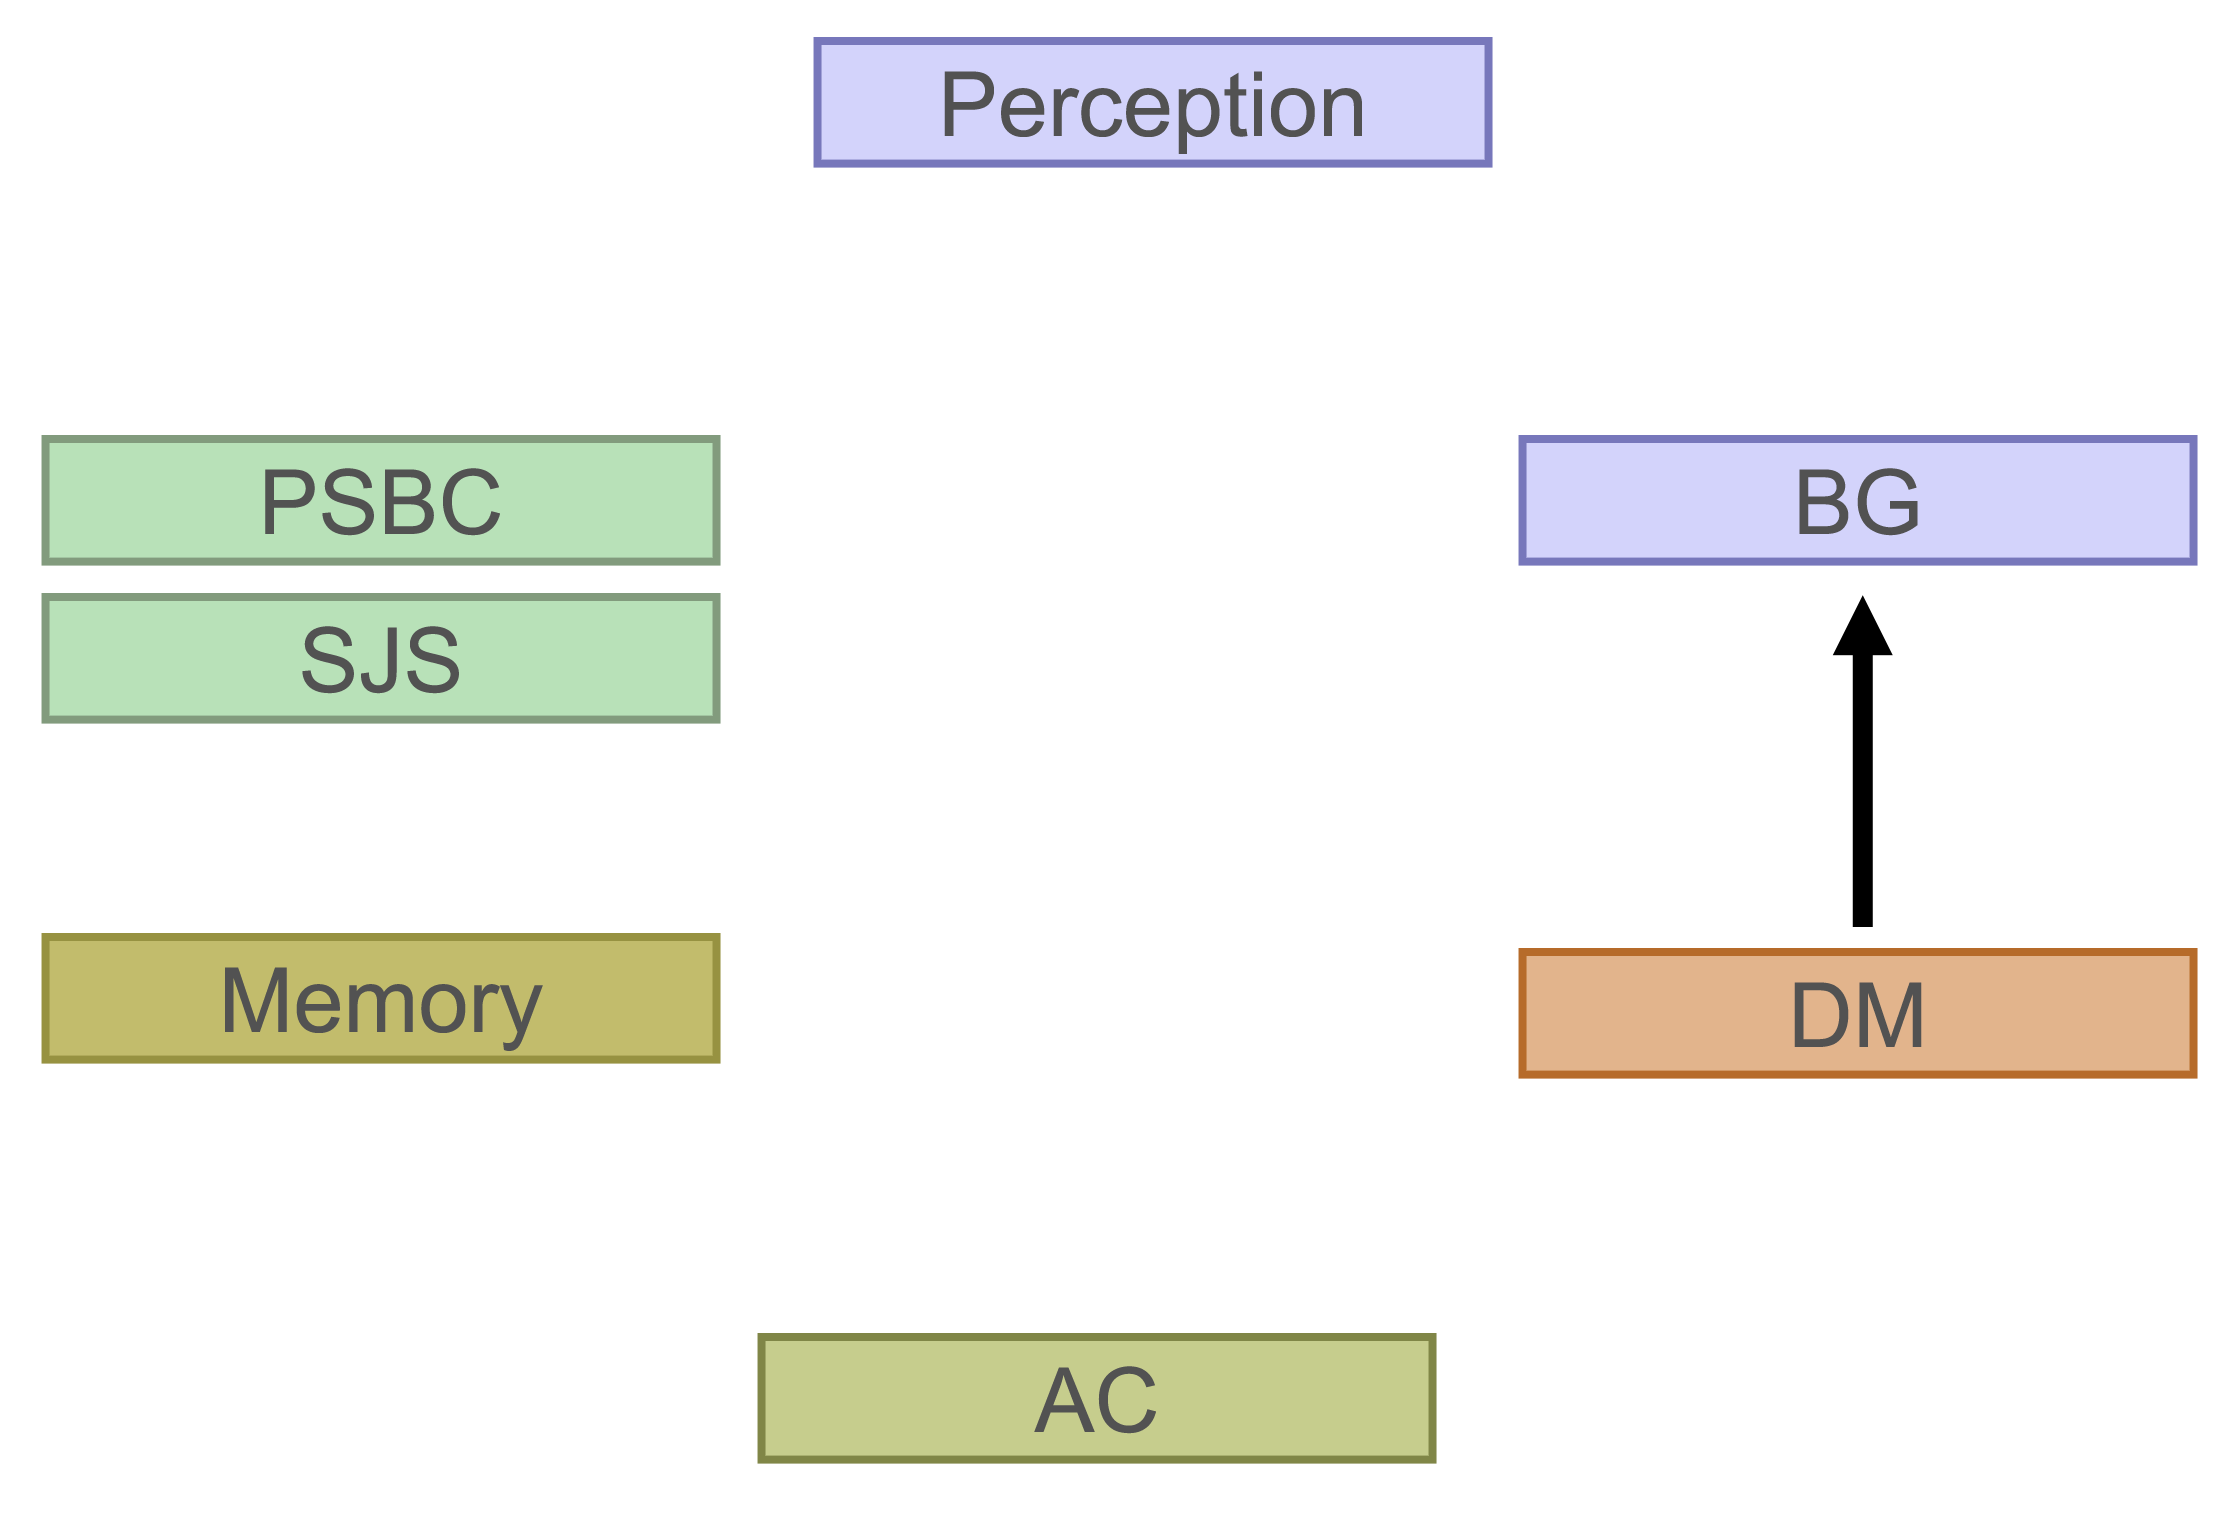
\includegraphics[width=0.8\textwidth]{plan_3.png}
      \end{center}
      
      Option 1: The \emph{Belief Generator} simulates the consequences.
   \end{frame}
   
   \begin{frame}{Architecture --- Agents}
      \begin{itemize}
         \item {How does this all fit together?}
      \end{itemize}
      
      \begin{center}
         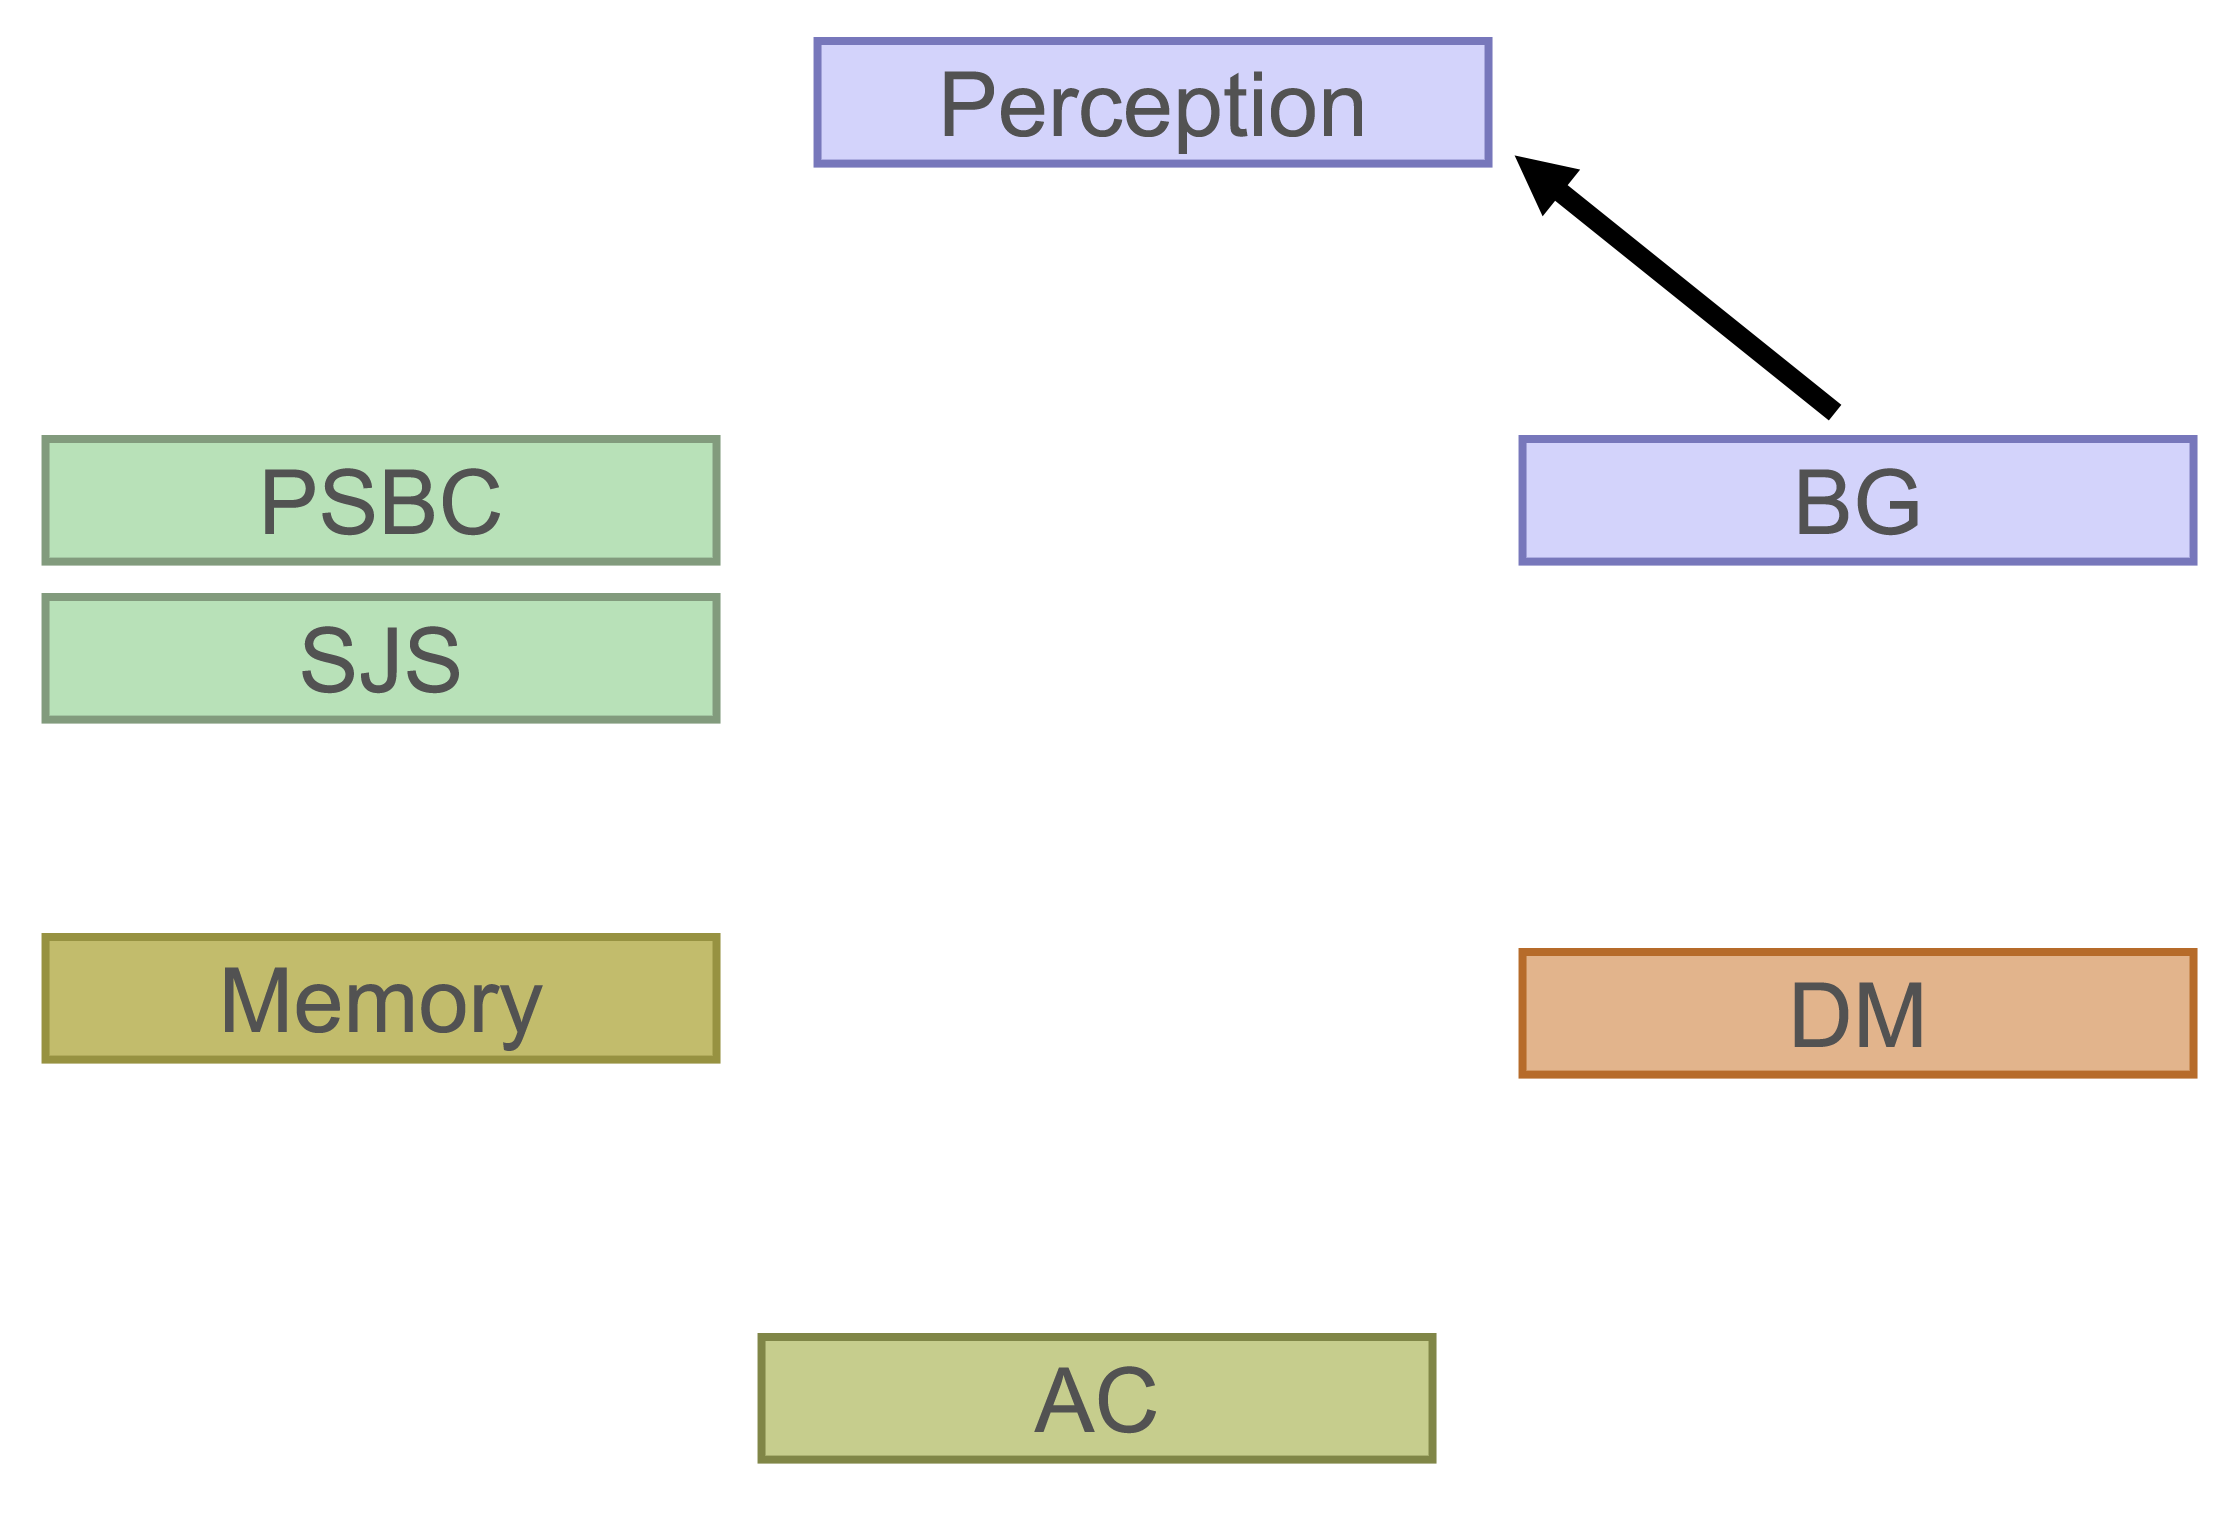
\includegraphics[width=0.8\textwidth]{plan_4.png}
      \end{center}
      
      The loop begins anew, but with \emph{imagined} perceptions.
   \end{frame}
   
   \begin{frame}{Architecture --- Agents}
      \begin{itemize}
         \item {How does this all fit together?}
      \end{itemize}
      
      \begin{center}
         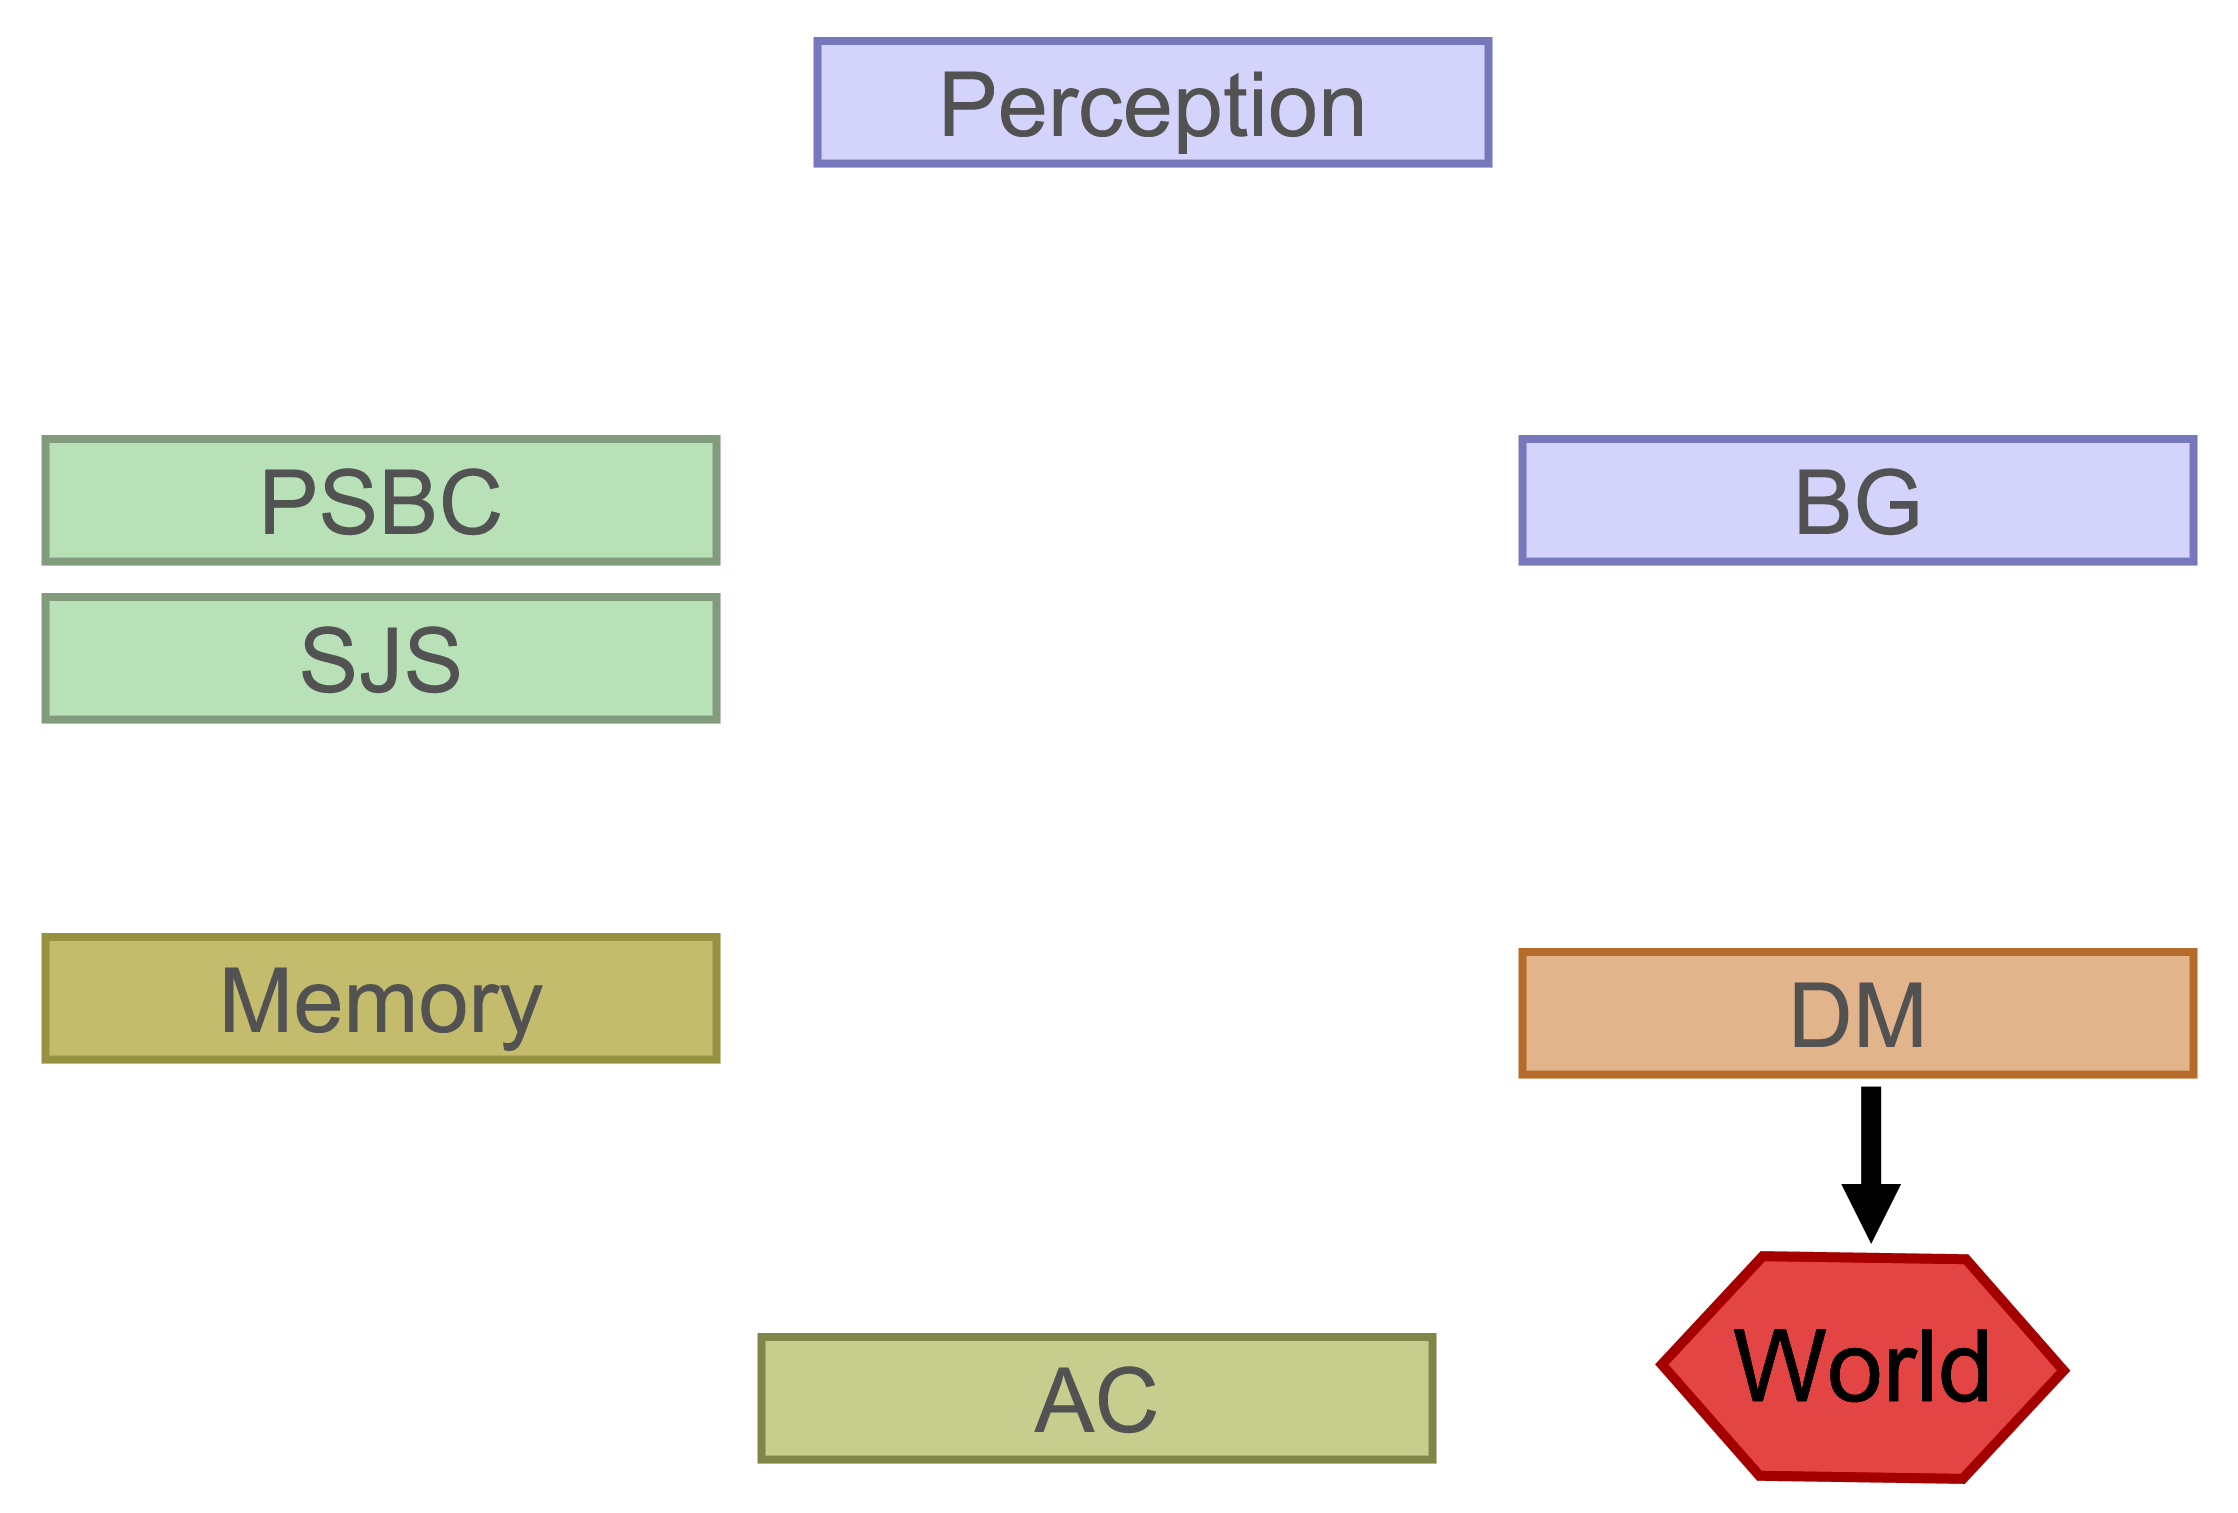
\includegraphics[width=0.8\textwidth]{plan_5.png}
      \end{center}
      
      Option 2: The \emph{Decision Maker} chooses a real action.
   \end{frame}
   
   \begin{frame}{Architecture --- Agents}
      \begin{itemize}
         \item To simplify it: DM and BG are in a loop.
      \end{itemize}
      
      \begin{center}
         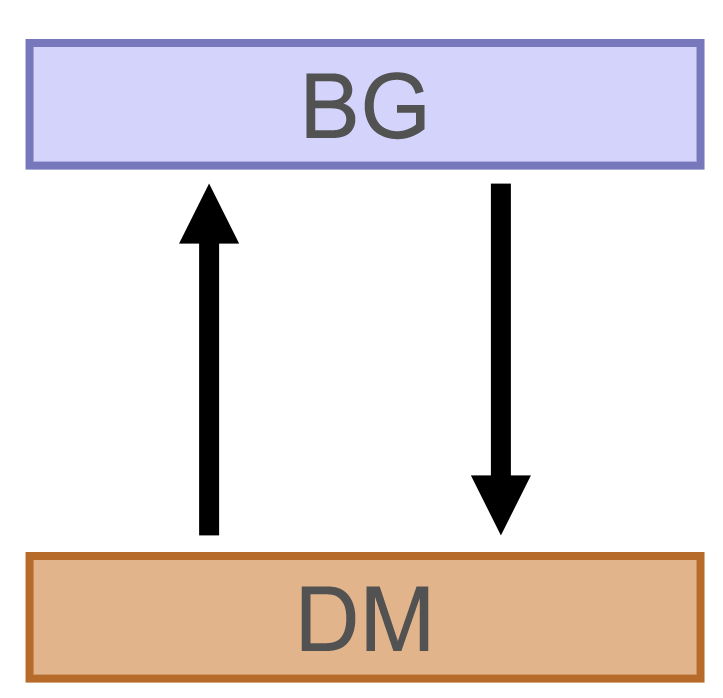
\includegraphics[width=0.3\textwidth]{bg_dm_loop.png}
      \end{center}
      
      \begin{enumerate}
         \item We choose a \emph{hypothetical} action,
         \item Then we simulate its consequences.
      \end{enumerate}
      
      \begin{itemize}
         \item We repeat this until the DM deems the outcome satisfactory and chooses a \emph{real} action.
      \end{itemize}
   \end{frame}
   
   \section{Results}
   
   \begin{frame}{Results}
      \begin{itemize}
         \item We created 32 populations with different personalities
         \item and simulated 50 rounds with each population.
         \item We combined weak/strong anger, fear, enthusiasm, contentment, as well as friendly/hostile demeanor.
         \item Throughout the simulation, we collected data: the number of
         \begin{itemize}
            \item gifts given,
            \item surviving Wumpuses,
            \item surviving agents,
            \item plants harvested, etc.
         \end{itemize}
      \end{itemize}
   \end{frame}
   
   \begin{frame}{Results}
      \begin{table}
         \centering
         \only<1>{%
         \begin{tabular}{ l | c | c }
            \emph{Personality fragment} & \emph{weak/hostile} & \emph{ strong/friendly} \\
            \hline
            Anger & 24.25 & 22.313\\
            Fear & 22.438 & 24.125\\
            Enthusiasm & 22.75 & 23.8125\\
            Contentment & 23.063 & 23.5\\
            Hostility & 23.625 & 22.938\\
            \hline
         \end{tabular}}
         \only<2>{%
            \begin{tabular}{ l | c | c }
               \emph{Personality fragment} & \emph{weak/hostile} & \emph{ strong/friendly} \\
               \hline
               \rowcolor{LightGreen} Anger & \cellcolor{IntenseGreen} 24.25 & 22.313\\
               Fear & 22.438 & 24.125\\
               Enthusiasm & 22.75 & 23.8125\\
               Contentment & 23.063 & 23.5\\
               Hostility & 23.625 & 22.938\\
               \hline
            \end{tabular}}
         \only<3>{%
            \begin{tabular}{ l | c | c }
               \emph{Personality fragment} & \emph{weak/hostile} & \emph{ strong/friendly} \\
               \hline
               \rowcolor{LightGreen} Anger & \cellcolor{IntenseGreen} 24.25 & 22.313\\
               \rowcolor{LightYellow} Fear & 22.438 & \cellcolor{IntenseYellow} 24.125\\
               Enthusiasm & 22.75 & 23.8125\\
               Contentment & 23.063 & 23.5\\
               Hostility & 23.625 & 22.938\\
               \hline
            \end{tabular}}
         \caption{Average number of surviving agents, by personality fragment.}
         \label{tab:numAgentsAvg}
      \end{table}
      
      \begin{itemize}
         \item<3-> Weak anger and strong fear are useful!
      \end{itemize}
   \end{frame}
   
   \begin{frame}{Results}
      \begin{itemize}
         \item Other surprising results:
      \end{itemize}
      
      \begin{table}
         \centering
            \begin{tabular}{ l | c }
               \emph{Personality} & \emph{Wumpuses} \\
               \hline

					$\personality{S}{W}{W}{W}{H}$ & 0\\
               \multicolumn{2}{c}{$\dots$}\\
               $\personality{W}{W}{W}{W}{H}$ & 0\\
               $\personality{S}{W}{W}{S}{F}$ & 1\\
               $\personality{S}{W}{W}{W}{F}$ & 2\\
               \multicolumn{2}{c}{$\dots$}\\
               $\personality{S}{W}{S}{W}{F}$ & 19\\
               $\personality{S}{W}{S}{W}{H}$ & 19\\
               \hline
            \end{tabular}
            \caption{Number of meat items given as gifts after 50 rounds.}
            \label{tab:numWumpuses}
      \end{table}
      
      \begin{itemize}
         \item $\personality{S}{W}{S}{W}{H}$ means ``strong anger, weak fear, strong enthusiasm, weak contentment, hostile demeanor''.
         \item Agents with strong anger and weak fear killed everything and shared the meat among themselves.
      \end{itemize}
   \end{frame}
   
   \section{Conclusion}
   
   \begin{frame}{Conclusion}
      \begin{itemize}
         \item We designed an agent architecture based on evolutionary considerations.
         \pause
         \item Our aim was to approximate real organisms.
         \pause
         \item Agents were put into a moderately complex game world
         \pause
         \item and performed reasonably well.
         \pause
         \item Personalities differentiated themselves in interesting ways.
      \end{itemize}
   \end{frame}
   
   \begin{frame}[plain, c]
      \begin{center}
         \huge Thank you for your attention!
      \end{center}
   \end{frame}
   
%   \begin{frame}
%      \frametitle{A Geometry Proof}
%      
%      (Illustrating {\sc beamer}'s $\backslash$uncover command.)
%      \vskip 0.5in
%      
%      \begin{theorem}
%         The angles in a triangle sum to $180^{\circ}$.
%      \end{theorem}
%      
%      \pause
%      
%      Plan:  Extend AC past C to D.  Draw CE parallel to AB.
%      
%   \end{frame}
   
%   \begin{frame}
%      \begin{proof}
%         \begin{tabular}{ll}
%            % uncover makes advanced overlay
%            \uncover<1->{1. u = y} & \uncover<2->{Alternate angles of a
%               transveral.} \\ 
%            \uncover<3->{2. v = x} & \uncover<4->{Consecutive interior angles of a
%               transveral} \\ 
%            \uncover<5->{3. z+u+v = $180^{\circ}$} & \uncover<6->{ACD is a straight
%               line.} \\ 
%            \uncover<7->{4. z+y+x = $180^{\circ}$} & \uncover<8->{Substitution
%               from Steps 1 and 2.} \\
%         \end{tabular}
%      \end{proof}
%   \end{frame}
\end{document}
